%%%%%%%%%%%%%%%%%%%%%%%%%%%%%%%%%%%%%%%%%%  不使用 authblk 包制作标题  %%%%%%%%%%%%%%%%%%%%%%%%%%%%%%%%%%%%%%%%%%%%%%
%-------------------------------PPT Title-------------------------------------
\title{材料智能计算与基础材料数据库}
%-----------------------------------------------------------------------------

%----------------------------Author & Date------------------------------------
\author[\textrm{Jun\_Jiang}]{姜\;\;骏\inst{}} %[]{} (optional, use only with lots of authors)
%% - Give the names in the same order as the appear in the paper.
%% - Use the \inst{?} command only if the authors have different
%%   affiliation.
\institute[BCC]{\inst{}%
%\institute[Gain~Strong]{\inst{}%
\vskip -20pt 北京市计算中心}
%\vskip -20pt {\large 格致斯创~科技}}
\date[\today] % (optional, should be abbreviation of conference name)
{	%{\fontsize{6.2pt}{4.2pt}\selectfont{\textcolor{blue}{E-mail:~}\url{jiangjun@bcc.ac.cn}}}
\vskip 45 pt {\fontsize{8.2pt}{6.2pt}\selectfont{%清华大学\;\;物理系% 报告地点
	\vskip 5 pt \textrm{2023.03.06}}}
}

%% - Either use conference name or its abbreviation
%% - Not really information to the audience, more for people (including
%%   yourself) who are reading the slides onlin%%   yourself) who are reading the slides onlin%%   yourself) who are reading the slides onlineee
%%%%%%%%%%%%%%%%%%%%%%%%%%%%%%%%%%%%%%%%%%%%%%%%%%%%%%%%%%%%%%%%%%%%%%%%%%%%%%%%%%%%%%%%%%%%%%%%%%%%%%%%%%%%%%%%%%%%%

\subject{}
% This is only inserted into the PDF information catalog. Can be left
% out.
%\maketitle
\frame
{
%	\frametitle{\fontsize{9.5pt}{5.2pt}\selectfont{\textcolor{orange}{“大数据中心调研座谈会”}}}
\titlepage
}
%-----------------------------------------------------------------------------

%------------------------------------------------------------------------------列出全文 outline ---------------------------------------------------------------------------------
%\section*{}
%\frame[allowframebreaks]
%{
%  \frametitle{Outline}
%%  \frametitle{\textcolor{mycolor}{\secname}}
%  \tableofcontents%[current,currentsection,currentsubsection]
%}
%%在每个section之前列出全部Outline
%%类似的在每个subsection之前列出全部Outline是\AtBeginSubsection[]
%\AtBeginSection[]
%{
%  \frame<handout:0>%[allowframebreaks]
%  {
%    \frametitle{Outline}
%%全部Outline中,本部分加亮
%    \tableofcontents[current,currentsection]
%  }
%}

%-----------------------------------------------PPT main Body------------------------------------------------------------------------------------
\small
\frame
{
	\frametitle{科学研究的范式变更}
\begin{figure}[h!]
\vspace*{-0.28in}
\centering
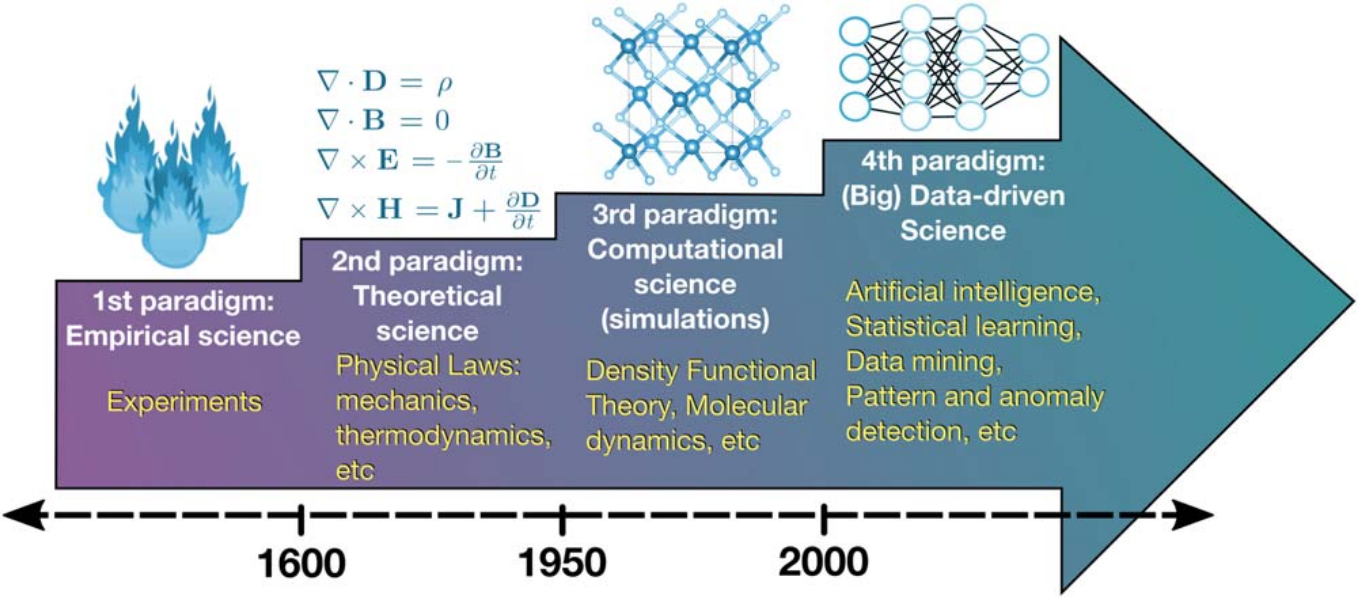
\includegraphics[height=2.00in,width=4.15in]{Figures/Four_Model_3.png}
%\caption{\tiny \textrm{Pseudopotential for metallic sodium, based on the empty core model and screened by the Thomas-Fermi dielectric function.}}%(与文献\cite{EPJB33-47_2003}图1对比)
\label{Four_Model}
\end{figure}
\begin{minipage}[b]{0.48\textwidth}
 {\fontsize{7.5pt}{6.0pt}\selectfont\begin{itemize}%[+-| alert@+>]
	 \setlength{\itemsep}{10pt}
 \item 逐步趋于理性
 \item 逐步趋于复杂
 \end{itemize}}
\end{minipage}
\hfill
\begin{minipage}[b]{0.48\textwidth}
 {\fontsize{7.5pt}{6.0pt}\selectfont\begin{itemize}%[+-| alert@+>]
	 \setlength{\itemsep}{10pt}
 \item 逐步趋于抽象
 \item 逐步趋于深刻
 \end{itemize}}
\end{minipage}
}

\begin{frame}{科学研究的重要助手:~计算模拟}
\begin{figure}[h!]
\vspace*{-0.18in}
\centering
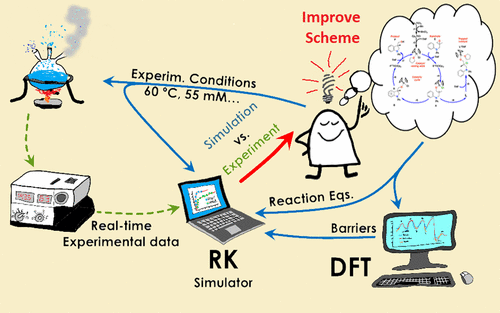
\includegraphics[height=2.55in,width=4.05in]{Figures/Schematic_Material-Design.png}
%\caption{\tiny \textrm{Pseudopotential for metallic sodium, based on the empty core model and screened by the Thomas-Fermi dielectric function.}}%(与文献\cite{EPJB33-47_2003}图1对比)
%\caption{\tiny \textrm{Pseudopotential for metallic sodium, based on the empty core model and screened by the Thomas-Fermi dielectric function.}}%(与文献\cite{EPJB33-47_2003}图1对比)
\label{Schematic_Material-Design}
\end{figure}
\end{frame}

\section{材料基因工程简介}
\frame
{
	\frametitle{材料基因工程}
\begin{figure}[h!]
\vspace*{-0.18in}
\centering
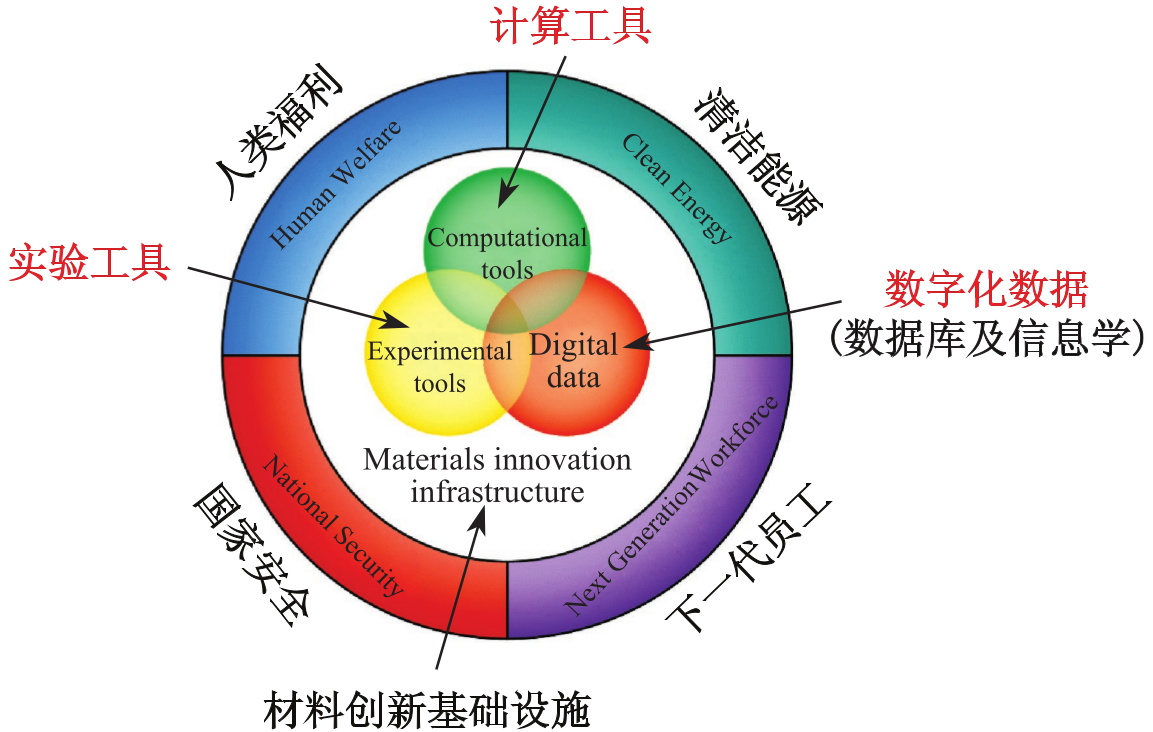
\includegraphics[height=2.55in,width=4.05in]{Figures/MGE.png}
%\caption{\tiny \textrm{Pseudopotential for metallic sodium, based on the empty core model and screened by the Thomas-Fermi dielectric function.}}%(与文献\cite{EPJB33-47_2003}图1对比)
%\caption{\tiny \textrm{Pseudopotential for metallic sodium, based on the empty core model and screened by the Thomas-Fermi dielectric function.}}%(与文献\cite{EPJB33-47_2003}图1对比)
\label{MGE}
\end{figure}
}

\frame
{
	\frametitle{材料模拟的基本思想和方法}
\begin{figure}[h!]
\vspace*{-0.25in}
\centering
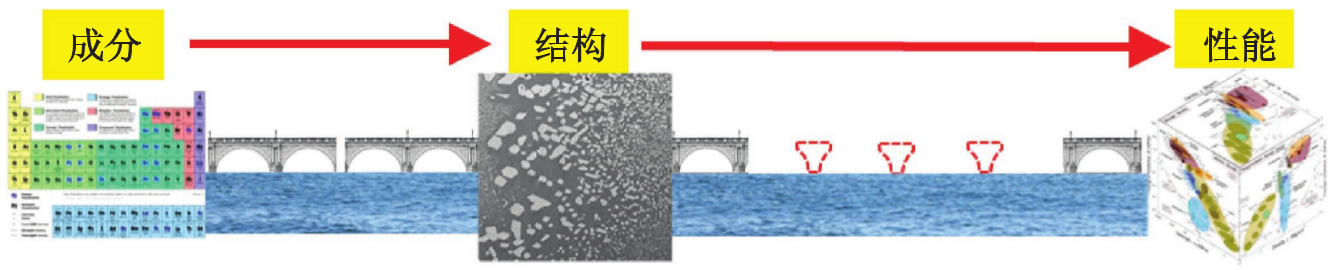
\includegraphics[height=0.80in,width=4.05in]{Figures/MGE-2.png}
%\caption{\tiny \textrm{Pseudopotential for metallic sodium, based on the empty core model and screened by the Thomas-Fermi dielectric function.}}%(与文献\cite{EPJB33-47_2003}图1对比)
\label{MGE}
\end{figure}
\begin{minipage}[c]{0.30\textwidth}
\begin{itemize}%[+-| alert@+>]
\vspace*{-2.25in}
 {\fontsize{7.5pt}{6.0pt}\selectfont
	 \setlength{\itemsep}{10pt}
 \item 变革研发模式,计算-实验-理论-数据科学相融合: 高效、低耗按需设计
 \item 数据驱动的材料创新平台主要面向复杂材料的模拟}
 \end{itemize}
\end{minipage}
\hfill
\begin{minipage}[b]{0.68\textwidth}
\begin{figure}[h!]
%\vspace*{-0.25in}
\centering
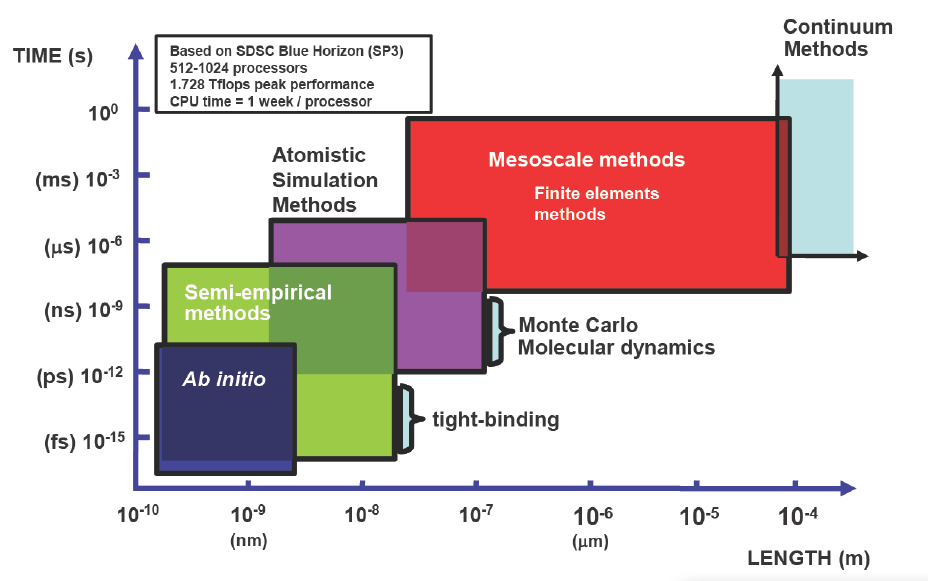
\includegraphics[height=1.60in,width=2.75in]{Figures/Multi-Scale-6.png}
%\caption{\tiny \textrm{Pseudopotential for metallic sodium, based on the empty core model and screened by the Thomas-Fermi dielectric function.}}%(与文献\cite{EPJB33-47_2003}图1对比)
\label{Multi-Scale}
\end{figure}
\end{minipage}
}

\begin{frame}
	\frametitle{材料基因工程推动新材料发展}
\begin{figure}[h!]
\vspace*{-0.25in}
\centering
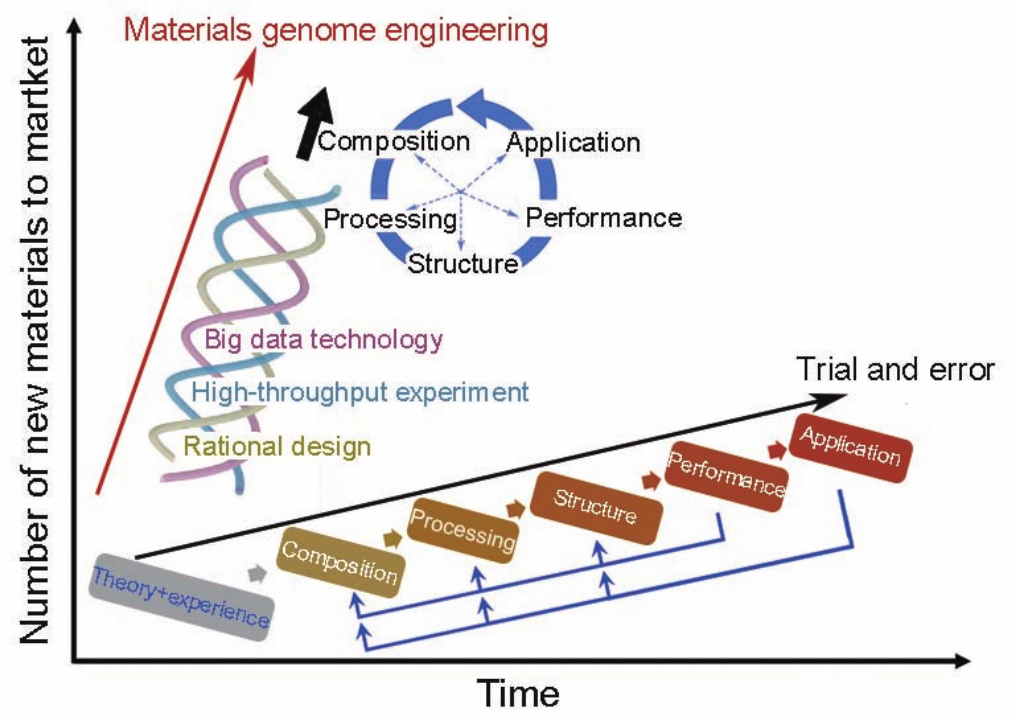
\includegraphics[height=2.90in,width=4.80in,viewport=0 0 1250 710,clip]{Figures/MGE_idea.png}
%\caption{\tiny \textrm{Pseudopotential for metallic sodium, based on the empty core model and screened by the Thomas-Fermi dielectric function.}}%(与文献\cite{EPJB33-47_2003}图1对比)
\label{MGE_idea}
\end{figure}
\end{frame}

\frame
{
	\frametitle{数据驱动的科学研究}
前所未有的计算能力和大规模的数据收集能力%,现代科学正在进入“第四范式”:
\begin{figure}[h!]
%\vspace*{-0.05in}
\centering
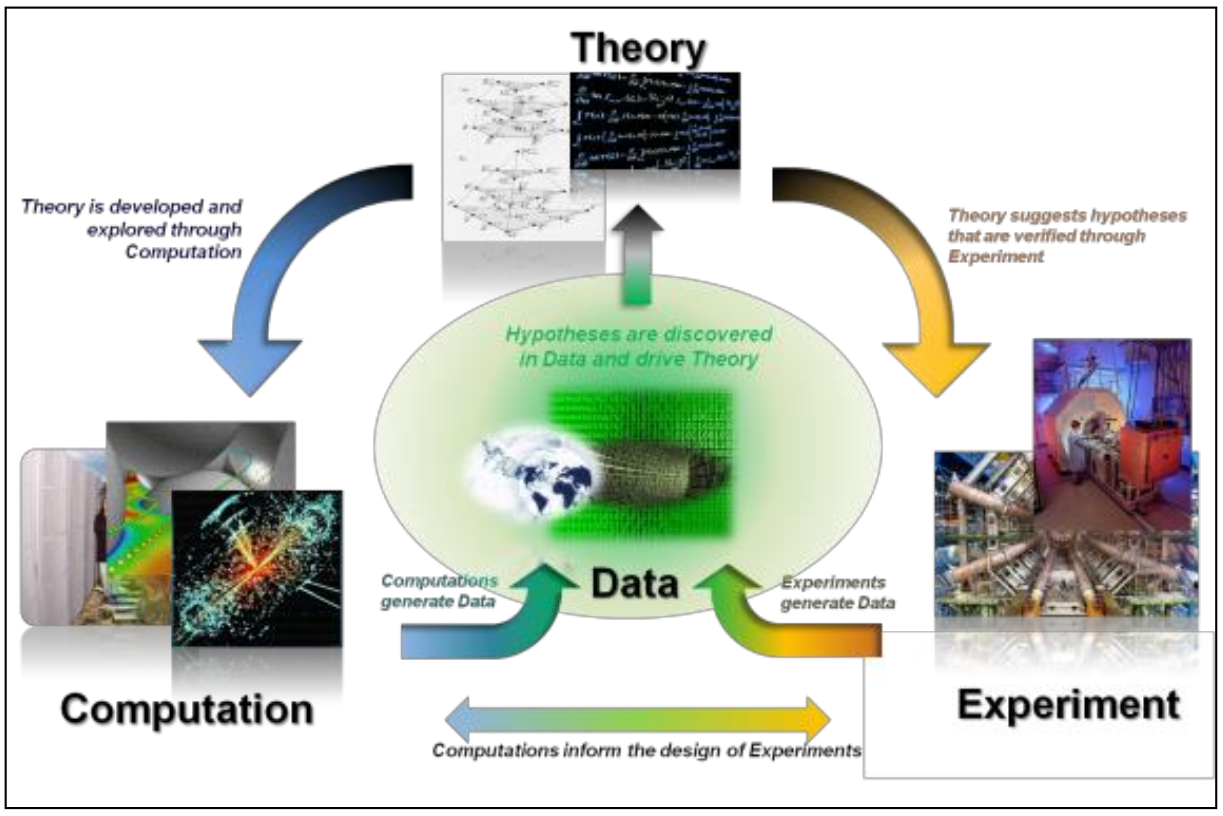
\includegraphics[height=2.40in,width=3.75in]{Figures/Four_Model_1.png}
%\caption{\tiny \textrm{Pseudopotential for metallic sodium, based on the empty core model and screened by the Thomas-Fermi dielectric function.}}%(与文献\cite{EPJB33-47_2003}图1对比)
\label{Four_Model_1}
\end{figure}
科学的新驱动力:~\textcolor{red}{密集数据}+\textcolor{red}{人工智能}\\
}

\section{高通量材料计算平台开发现状}     %Bookmark
\frame
{
	\frametitle{国外已有的计算平台}
\begin{figure}[h!]
\centering
\vspace{-15.5pt}
\subfigure[\fontsize{7.5pt}{6.2pt}\selectfont{\textrm{Auto-FLOW (AFLOW)}\upcite{CMS58-227_2012}}]{
\label{AFLOW_data_flow}
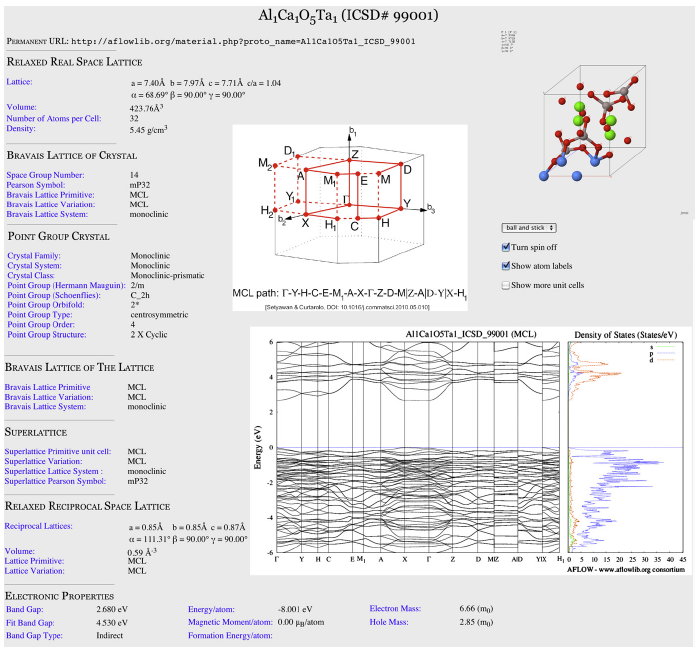
\includegraphics[height=1.2in,width=1.6in,viewport=0 0 720 660,clip]{Figures/AFLOW_database.png}}
\subfigure[\fontsize{7.5pt}{6.2pt}\selectfont{\textrm{Material Project (MP)}\upcite{CMS97-209_2015}}]{
\label{MP_commp_infrastructure}
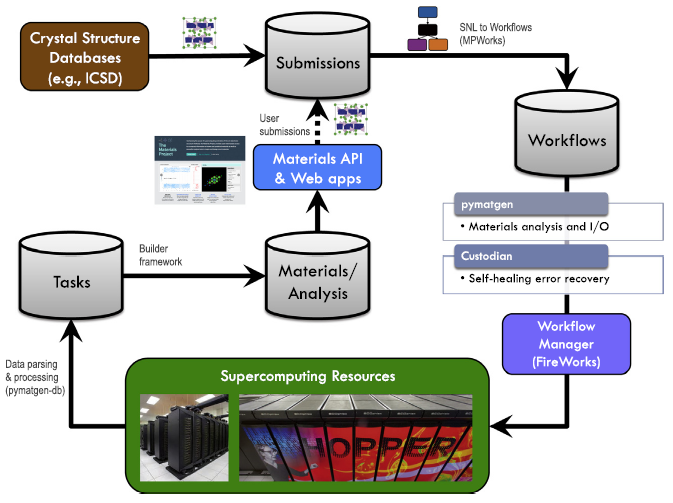
\includegraphics[height=1.2in,width=1.7in,viewport=0 0 670 530,clip]{Figures/MP_comp_infrastructure.png}}
\subfigure[\fontsize{3.5pt}{3.2pt}\selectfont{\textrm{Quantum Materials Informatics Project (QMIP)}\upcite{url_QMIP}}]{
\label{QMIP_Shame}
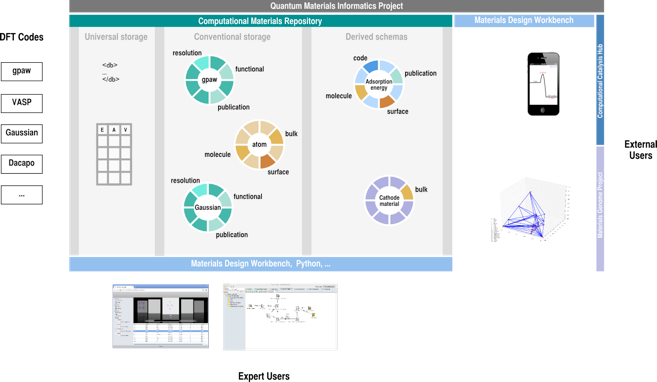
\includegraphics[height=1.2in,width=1.7in,viewport=0 0 670 420,clip]{Figures/QMIP_shame.png}}
\subfigure[\fontsize{6.5pt}{5.2pt}\selectfont{\textrm{Clean Energy Project (CEP)}\upcite{JPCL2-2241_2011}}]{
\label{CEP_structure_flow}
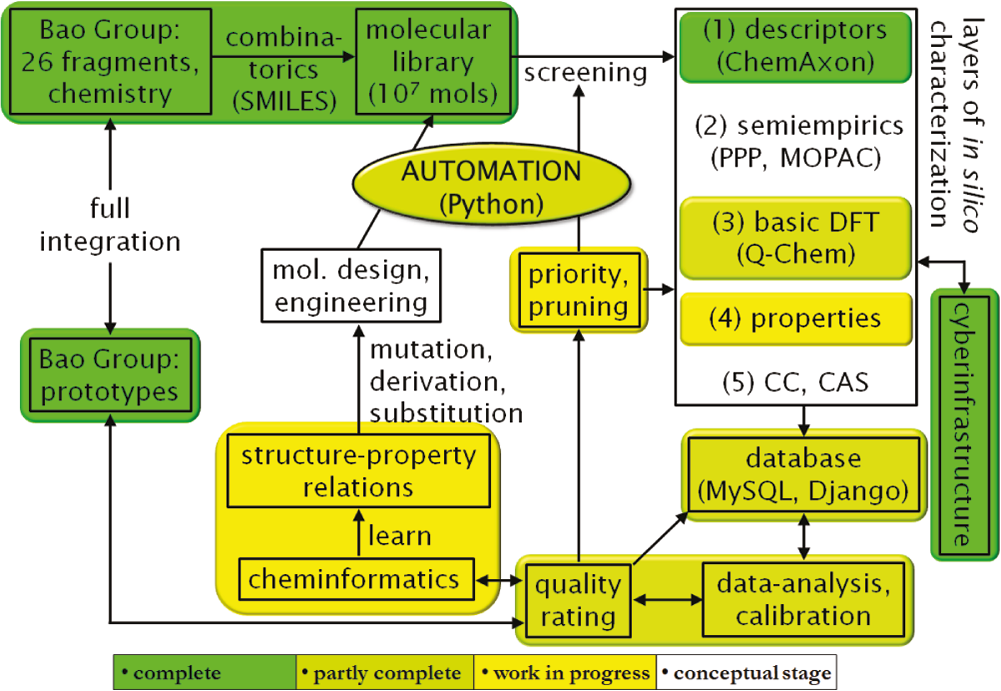
\includegraphics[height=1.2in,width=1.6in,viewport=0 0 1020 730,clip]{Figures/CEP_structure_flow.png}}
%\caption{}%
\label{Auto_Flow_Platform-1}
\end{figure}
}

\frame
{
	\frametitle{\textrm{ASE}:~接口丰富的适应性计算平台}
\begin{figure}[h!]
\centering
\vspace*{-0.2in}
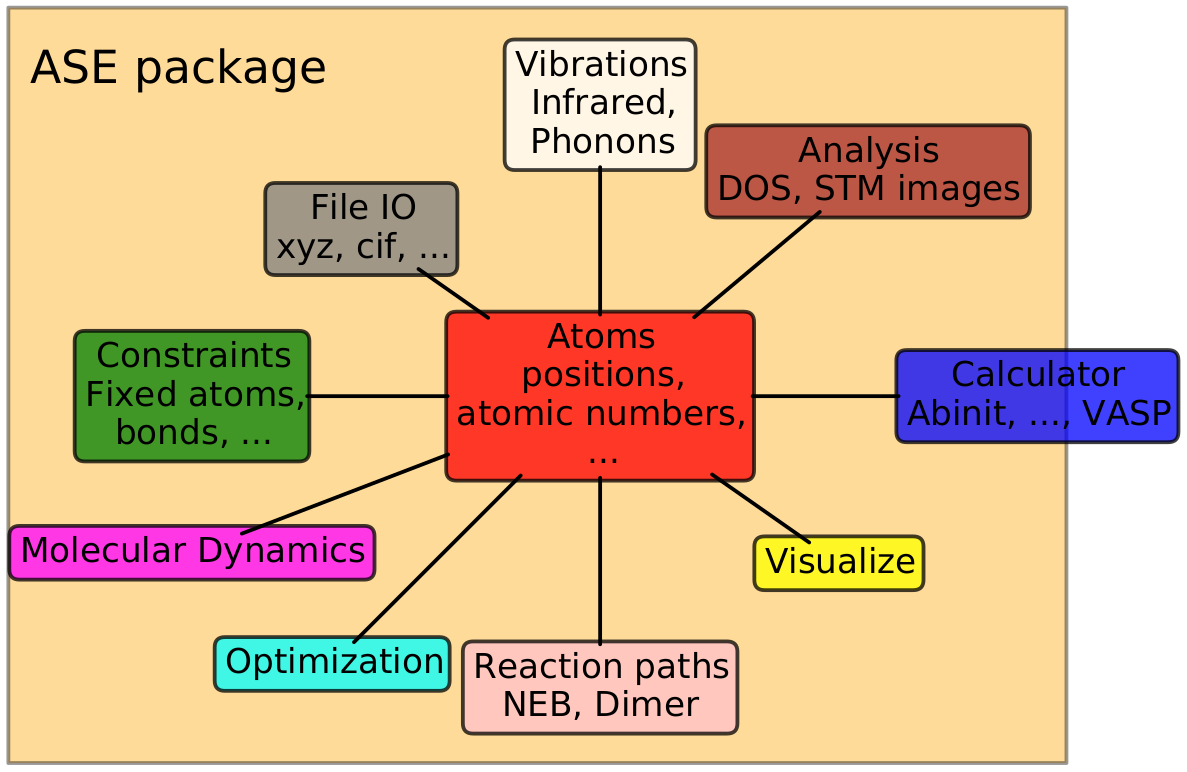
\includegraphics[height=2.5in,width=4.0in,viewport=0 0 1208 830,clip]{Figures/ASE_Python_lib.png}
\caption{\fontsize{7.2pt}{4.2pt}\selectfont{\textrm{ASE:~a Python library for working with atoms.}}}%
\label{Logo_ASE_lib}
\end{figure} 
}

\frame
{
	\frametitle{国内已有的计算平台:~\textrm{MatCloud}}
\begin{figure}[h!]:
\centering
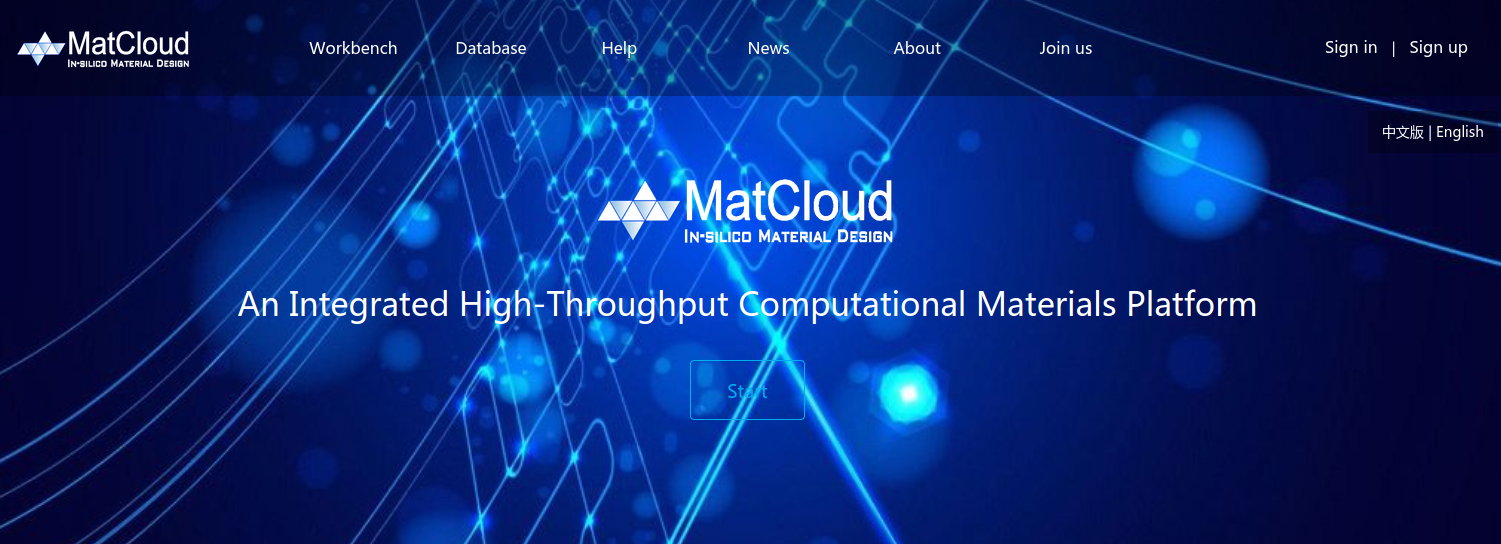
\includegraphics[height=1.57in,width=4.95in,viewport=0 0 1800 550,clip]{Figures/Matcloud-login.png}
\caption{\fontsize{7.2pt}{4.2pt}\selectfont{中科院计算机网络信息中心~杨小渝团队开发}\upcite{CMS146-319_2018,url_Matcloud}}%
\label{Auto_Flow_Platform-2}
\end{figure}
}

\frame
{
	\frametitle{\textrm{Atomly}:~物理所的无机晶体材料计算数据库}
\begin{figure}[h!]
\centering
\vspace*{-0.2in}
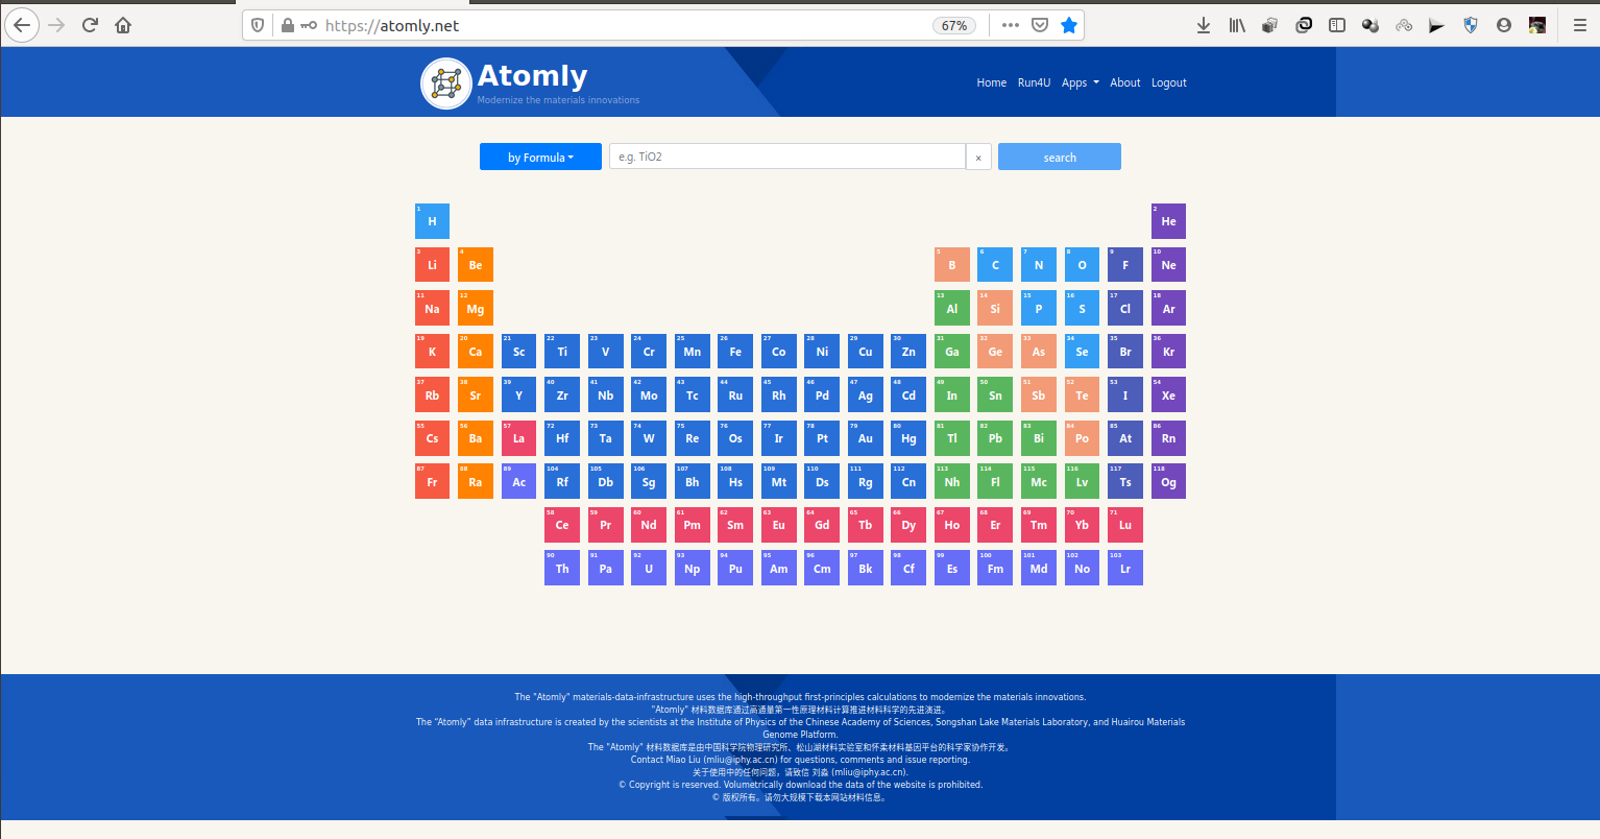
\includegraphics[height=2.1in,width=4.1in,viewport=5 0 1608 830,clip]{Figures/Atomly.png}
\caption{\fontsize{7.2pt}{4.2pt}\selectfont{\textrm{Atomly:~中科院物理所~刘淼等老师开发,数据库包含了17万\!$^+$\!无机晶体材料第一性原理计算结果\textrm{(包含电子结构信息:~DOS~+~energy~bands)}.}}}%
\label{Logo_Atomly_lib}
\end{figure} 
}

\frame
{
	\frametitle{\textrm{计算平台的功能和总体架构}}
\begin{figure}[h!]
\centering
\vspace*{-0.35in}
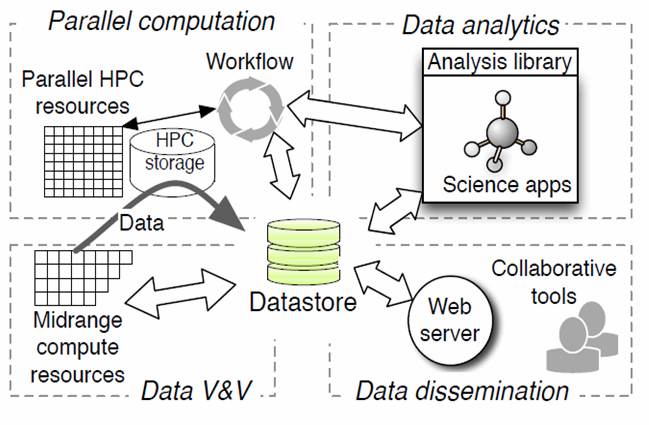
\includegraphics[height=2.6in,width=4.05in,viewport=0 0 670 460,clip]{Figures/Parallel_computation.png}
%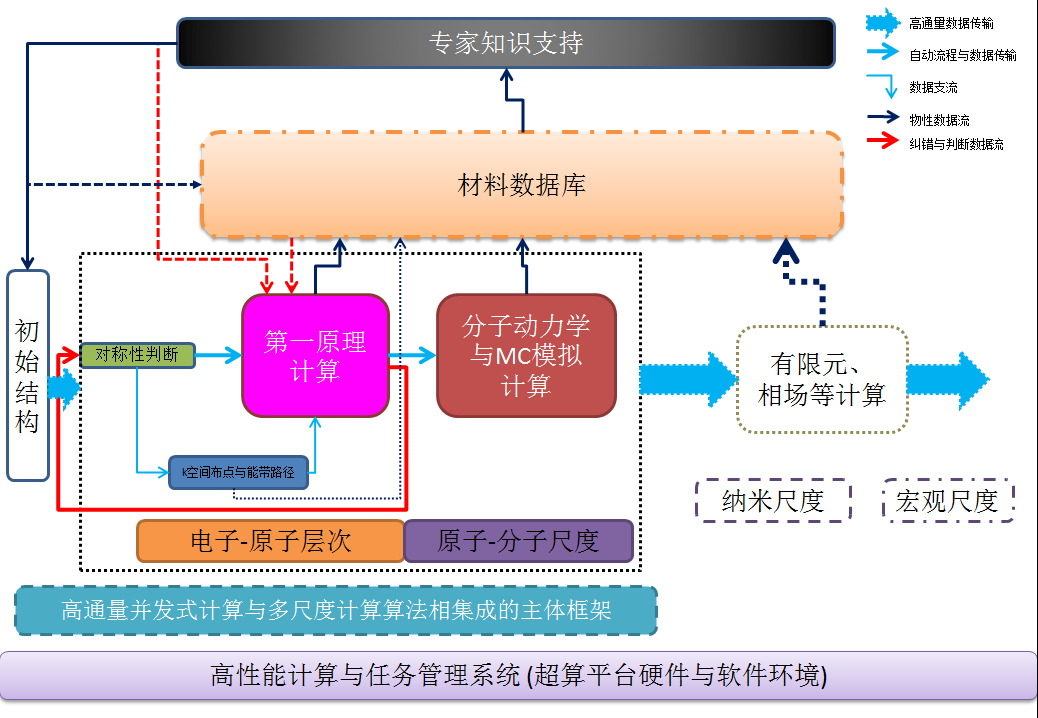
\includegraphics[height=1.6in,width=2.4in,viewport=0 0 1038 730,clip]{Figures/Auto_Flow.png}
\caption{\fontsize{7.2pt}{4.2pt}\selectfont{\textrm{The schematic framework and platform of all those project.}}}%
\label{Auto_Flow}
\end{figure} 
}

%\frame
%{
%	\frametitle{现有高通量计算平台概览}
%\begin{table}[!h]
%\tabcolsep 0pt \vspace*{-12pt}
%%\caption{}
%\label{Table-Cost}
%\begin{minipage}{0.85\textwidth}
%%\begin{center}
%\centering
%\def\temptablewidth{1.1\textwidth}
%\renewcommand\arraystretch{0.8} %表格宽度控制(普通表格宽度的两倍)
%\rule{\temptablewidth}{1pt}
%\begin{tabular*} {\temptablewidth}{@{\extracolsep{\fill}}c@{\extracolsep{\fill}}c@{\extracolsep{\fill}}c@{\extracolsep{\fill}}c@{\extracolsep{\fill}}c@{\extracolsep{\fill}}c@{\extracolsep{\fill}}c}
%%-------------------------------------------------------------------------------------------------------------------------
%	&\multirow{2}{*}{\fontsize{7.2pt}{5.2pt}\selectfont{编程语言}}	&\fontsize{7.2pt}{5.2pt}\selectfont{建模} &\multicolumn{2}{|c|}{\fontsize{6.2pt}{5.2pt}\selectfont{任务提交与管理}} &\multirow{2}{*}{\fontsize{7.2pt}{5.2pt}\selectfont{后处理}} &\multirow{2}{*}{\fontsize{6.2pt}{5.2pt}\selectfont{数据组织管理}} \\\cline{4-5}
%	&	&\fontsize{7.2pt}{5.2pt}\selectfont{功能} &\multicolumn{1}{|l}{\fontsize{7.2pt}{5.2pt}\selectfont{软件接口}} &\multicolumn{1}{r|}{\fontsize{7.2pt}{5.2pt}\selectfont{运行容错}} & & \\\hline
%	\fontsize{7.2pt}{5.2pt}\selectfont{{AFLOW}} &\fontsize{7.2pt}{5.2pt}\selectfont{C++} &\checkmark &\triangle &\FiveStarOpen &\FiveStarOpen &\fontsize{7.2pt}{5.2pt}\selectfont{{Django}} \\
%	\fontsize{7.2pt}{5.2pt}\selectfont{{MP}} &\fontsize{7.2pt}{5.2pt}\selectfont{Python} &\checkmark &\checkmark &\FiveStarOpen &\FiveStarOpen &\fontsize{7.2pt}{5.2pt}\selectfont{{MongoDB}} \\
%	\multirow{2}{*}{\fontsize{7.2pt}{5.2pt}\selectfont{{QMIP}}} &\fontsize{7.2pt}{5.2pt}\selectfont{JavaScript/SVG} &\multirow{2}{*}{\checkmark} &\multirow{2}{*}{\checkmark} &\multirow{2}{*}{--} &\multirow{2}{*}{\checkmark} &\multirow{2}{*}{--} \\
%	&\fontsize{7.2pt}{5.2pt}\selectfont{+html/Python} & & & & & \\
%	\fontsize{7.2pt}{5.2pt}\selectfont{{CEP}} &\fontsize{7.2pt}{5.2pt}\selectfont{Python} &\checkmark &\checkmark &-- &\checkmark &\fontsize{7.2pt}{5.2pt}\selectfont{{Django/MySQL}} \\
%	\fontsize{7.2pt}{5.2pt}\selectfont{{ASE}} &\fontsize{7.2pt}{5.2pt}\selectfont{Python} &\FiveStarOpen &\FiveStarOpen &-- &\triangle &-- \\
%	\multirow{2}{*}{\fontsize{7.2pt}{5.2pt}\selectfont{{MatCloud}}} &\fontsize{7.2pt}{5.2pt}\selectfont{JavaScript} &\multirow{2}{*}{\checkmark} &\multirow{2}{*}{\triangle} &\multirow{2}{*}{\checkmark} &\multirow{2}{*}{\checkmark} &\multirow{2}{*}{\fontsize{7.2pt}{5.2pt}\selectfont{{MongoDB}}} \\
%	&\fontsize{7.2pt}{5.2pt}\selectfont{+.NETCore} & & & & &
%\end{tabular*}
%\rule{\temptablewidth}{1pt}
%\end{minipage}
%%\vskip -15pt
%\fontsize{7.2pt}{5.2pt}\selectfont{
%\begin{description}
%	\item[\FiveStarOpen]~该功能较突出
%	\item[\checkmark]~该功能基本满足需求
%	\item[\triangle]~该功能存在不足
%\end{description}}
%%\end{center}
%\end{table}
%\fontsize{8.2pt}{6.2pt}\selectfont{
%	\textrm{Lin L. \textit{Materials databases infrastructure constructed by first principles calculations:~a review.} \textbf{Mater. Perform. Character.}, 2015, 4(1):148.}}
%}

\section{\rm{MP}与\rm{ASE}}     %Bookmark
\frame
{
	\frametitle{\textrm{MP}自动流程的设计与开发}
	\begin{itemize}
		\item \textcolor{red}{设计目标}:~围绕\textrm{VASP~}作业高通量并发提交与过程监控
		\item \textcolor{red}{设计方案}:~开发针对不同计算场景的功能模块
			\begin{enumerate}
    \setlength{\itemsep}{15pt}
				\item \textcolor{blue}{\textbf{Pymatgen}}\\
					\textcolor{magenta}{前处理}:~计算模型的分析与预处理\\
					\textcolor{magenta}{后处理}:~计算结果的可视化
				\item \textcolor{blue}{\textbf{FireWorks}}\\
\textcolor{magenta}{计算流程设计与管理}:~数据库支持的计算流程管理
				\item \textcolor{blue}{\textbf{Custodian}}\\
\textcolor{magenta}{计算流程容错与应对}:~提供计算过程错误判断接口,由用户提供解决策略和针对性设计
			\end{enumerate}
	\end{itemize}
		%\item 计算过程的控制方式
}

\frame
{
	\frametitle{\textrm{Pymatgen}的模块结构}
\begin{figure}[h!]
\centering
\vspace*{-0.1in}
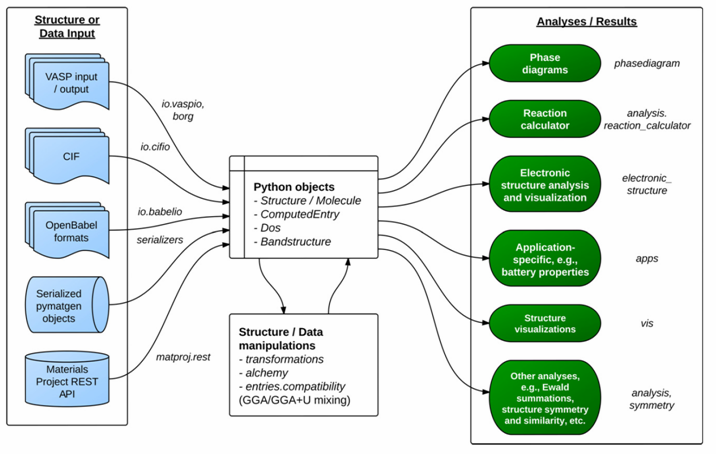
\includegraphics[height=2.3in]{Figures/MP_library.png}
\caption{\fontsize{7.2pt}{4.2pt}\selectfont{\textrm{Overview of a typical workflow for pymatgen.}}}%
\label{Pymatgen_Lib}
\end{figure} 
}

\frame
{
	\frametitle{\textrm{Pymatgen}可展示的材料物性}
\begin{figure}[h!]
\centering
\vspace*{-0.1in}
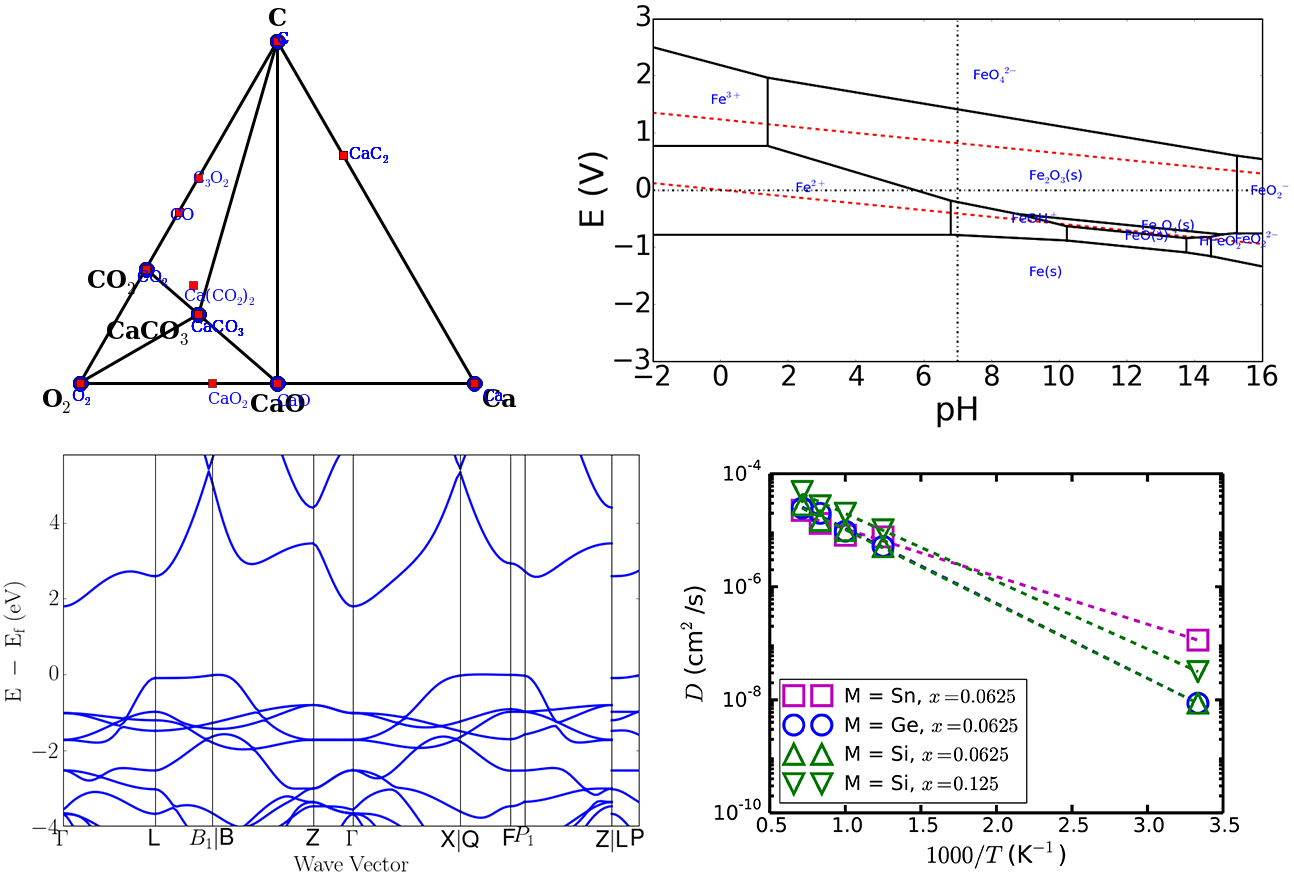
\includegraphics[height=2.3in]{Figures/MP_vision.png}
\caption{\fontsize{5.2pt}{4.2pt}\selectfont{\textrm{Top left: Phase; Top right: Pourbaix diagram from the Materials API. \\Bottom left: Calculated bandstructure plot using pymatgen’s parsing and plotting utilities. Bottom right: Arrhenius plot using pymatgen’s Diffusion~Analyzer.}}}%
\label{Pymatgen_vision}
\end{figure} 
}

\frame
{
	\frametitle{\textrm{FireWorks}的模块结构}
\textrm{FireWorks}发布的工作流成由三层嵌套结构组成:
\fontsize{8.2pt}{6.2pt}\selectfont{
\begin{itemize}
	\item \textrm{Firetask}:~基本执行单元,是执行计算的最基本脚本命令或\textrm{Python}命令。
	\item \textrm{Firework}:~组织基本执行单元构成任务单元组,并指定各基本执行单元所需的参数。
	\item \textrm{Workflow}:~彼此相关联的任务单元组构成完整的工作流程:\\
		\textrm{FireWork}之间的数据传递、任务执行序列等由\textrm{FWAction}完成。
\end{itemize}}
\begin{figure}[h!]
\centering
\vspace*{-0.1in}
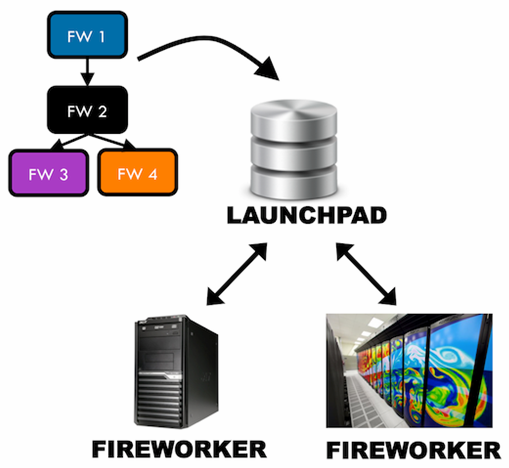
\includegraphics[height=1.5in]{Figures/MP_fireworks.png}
\hskip 1pt
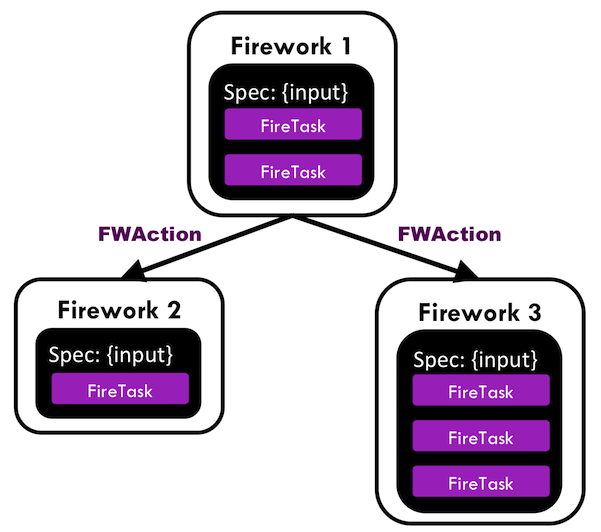
\includegraphics[height=1.5in]{Figures/MP_multiple_fw.png}
\caption{\fontsize{7.2pt}{4.2pt}\selectfont{\textrm{The basic infrastructure of FireWorks.}}}%
\label{FireWorks_FW}
\end{figure} 
}

\frame
{
	\frametitle{\textrm{FireWorks}的模块结构}
\fontsize{8.2pt}{6.2pt}\selectfont{
	\begin{itemize}
		\item \textrm{FireWorks}是以任务单元组为基本组成的来实现工作流程的,任务单元组之间依靠数据传递相关联,流程执行完毕也将返回数据,\textrm{FWAction}模块主要负责任务单元组之间的数据传递和任务分配。
		\item \textrm{FWAction}允许用户根据需要设计和更改流程参数、增添、删减和改变流程(子)单元组,这一模块大大增加了\textrm{FireWorks}工作流的灵活性。
	\end{itemize}}
\begin{figure}[h!]
\centering
\vspace*{-0.10in}
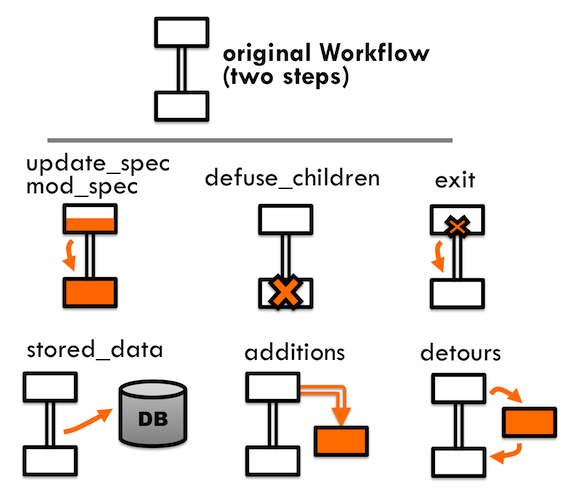
\includegraphics[height=1.9in]{Figures/MP_Fireworks_fwactions.png}
\caption{\fontsize{7.2pt}{4.2pt}\selectfont{\textrm{FireWorks}的单元组间数据传递与处理示意.}}%
\label{FireWorks_FWA}
\end{figure} 
}

\frame
{
	\frametitle{\textrm{FireWorks}的模块结构}
这种“发布-执行”结构使得计算任务与软件、硬件高度解耦,用户可根据需要随时向\textrm{LaunchPad}添加新的工作流,承担计算任务的\textrm{FireWorkers}彼此也可以是完全异构的,具有很好的机动性。
\vskip 0.25in
对于材料第一原理计算自动流程而言,一个\textrm{DFT}计算过程就是一个\textrm{Firework},可以分解为:
\begin{enumerate}
	\item 指定计算控制参数(参数在数据库中\texttt{Json}存储,由\textrm{Spec}传入)
	\item 计算控制文件生成(每个\textrm{Firetask}生成一个控制文件)
	\item \textrm{DFT}计算作业提交(一个\textrm{Firetask})
\end{enumerate}
在此基础上,可以通过\textrm{FWAction}修改控制参数,将\textrm{DFT}计算单元组组织成完整的材料第一原理计算流程,并将最终结果直接导入材料计算数据库。
}

\frame
{
	\frametitle{\textrm{Custodian}的容错逻辑}
\begin{figure}[h!]
\centering
\vspace*{-0.1in}
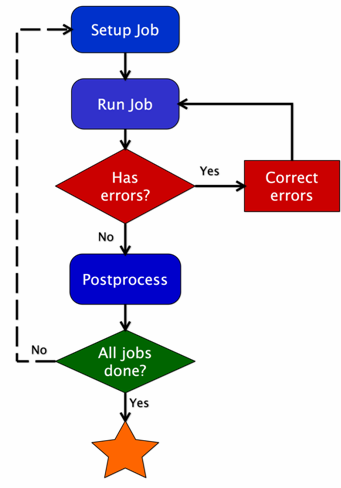
\includegraphics[height=2.7in]{Figures/MP_custodian.png}
\label{Custodian_over}
\caption{\fontsize{7.2pt}{4.2pt}\selectfont{\textrm{Overview of the Custodian workflow.}}}%
\end{figure} 
}

\frame
{
	\frametitle{\textrm{atomate}:~计算流程控制示范}
%		\textcolor{purple}{\textrm{Atomate}}:~:~适合一定复杂程度的\textrm{~VASP~}计算
\begin{figure}[h!]
\centering
\vspace*{-0.19in}
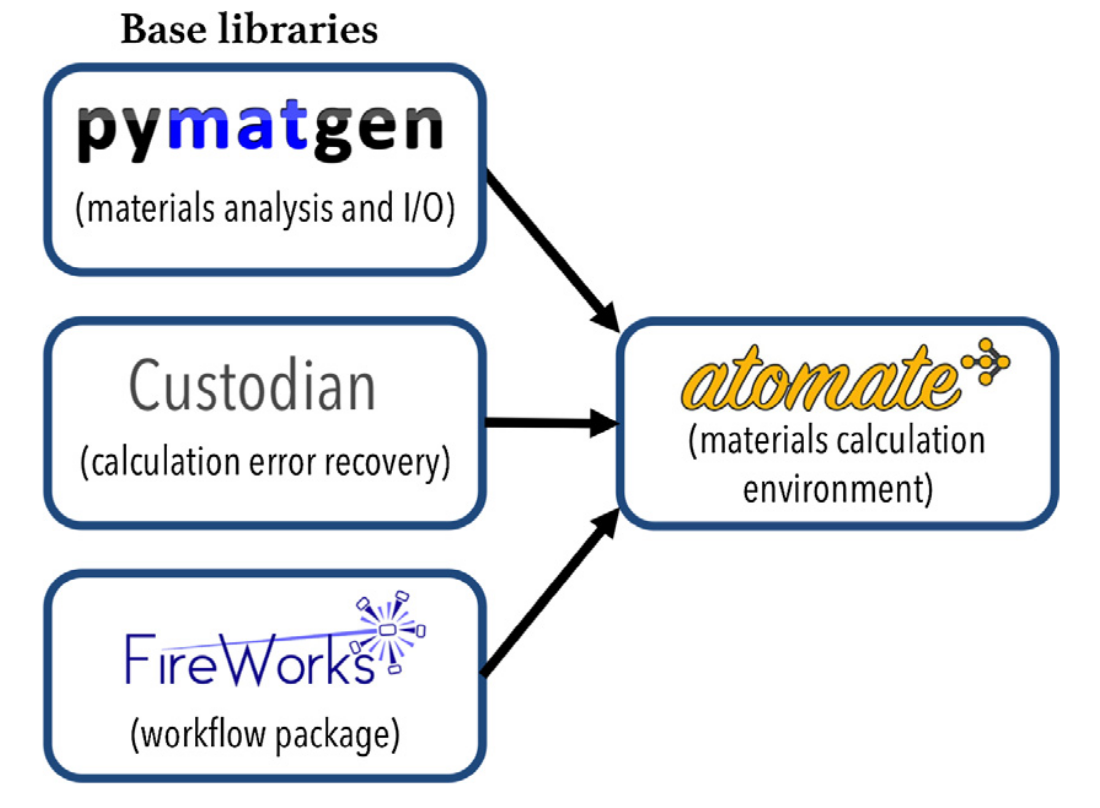
\includegraphics[height=1.4in,width=2.2in,viewport=0 0 820 630,clip]{Figures/Atomate_comp.png}
\vskip 1pt
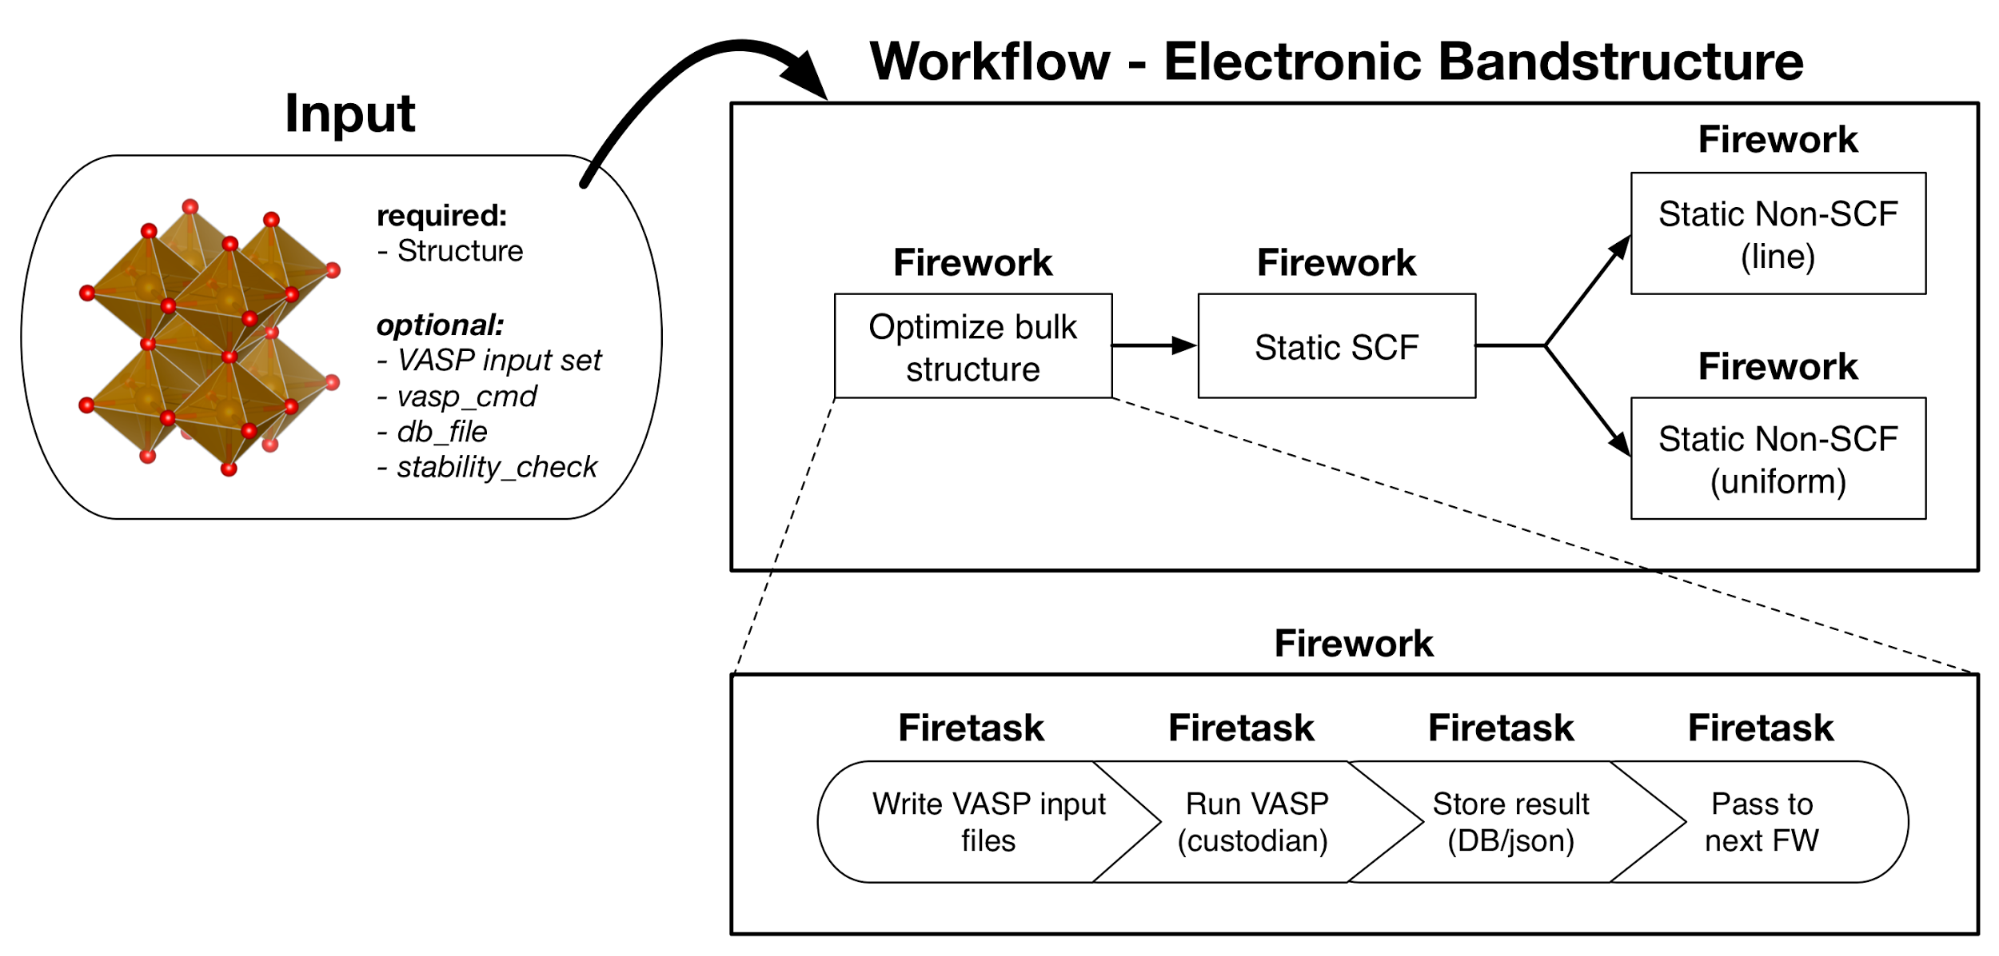
\includegraphics[height=1.5in]{Figures/bandstructure_wf.png}
%\caption{\fontsize{7.2pt}{4.2pt}\selectfont{\textrm{The integrated calculator in ASE (Atomic Simulation Environment).}}}%
\label{Logo_QM-MM}
\end{figure} 
}

\frame
{
	\frametitle{\textrm{ASE}自动流程的设计与管理}
		\textcolor{purple}{\textrm{ASE}}:~模块加载式计算流程控制,更符合复杂多尺度计算场景
		\begin{itemize}
			\item \textcolor{magenta}{灵活的建模功能}
				\begin{enumerate}
    \setlength{\itemsep}{10pt}
					\item 简单堆积:~原子直接组成分子
					\item 理想周期体系(包括一维、二维、三维)
					\item 表面和表面吸附,可指定吸附位
				\end{enumerate}
			\item \textcolor{magenta}{丰富的软件接口}\\
				提供了包括绝大部分第一原理和分子动力学计算软件接口,方便组合实现多尺度计算
			\item \textcolor{magenta}{不依赖软件的优化与动力学模拟}\\
				适合复杂材料物性模拟的优化和多种动力学过程模拟
			\item \textcolor{magenta}{多样化的数据库类型}
		\end{itemize} 
}

\frame
{
\frametitle{\textrm{ASE}特色:~材料结构生成模块}
\begin{figure}[h!]
\centering
\vspace*{-0.15in}
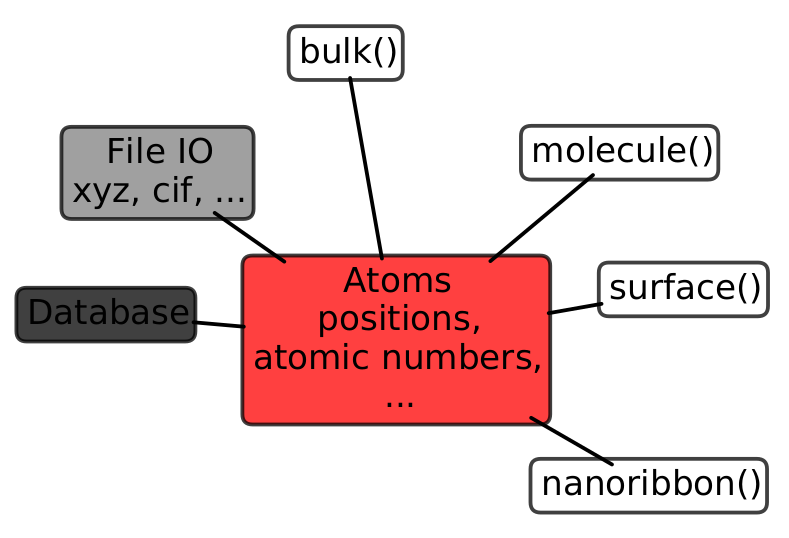
\includegraphics[height=1.2in,width=1.7in,viewport=0 0 820 530,clip]{Figures/ASE_atoms_module.png}
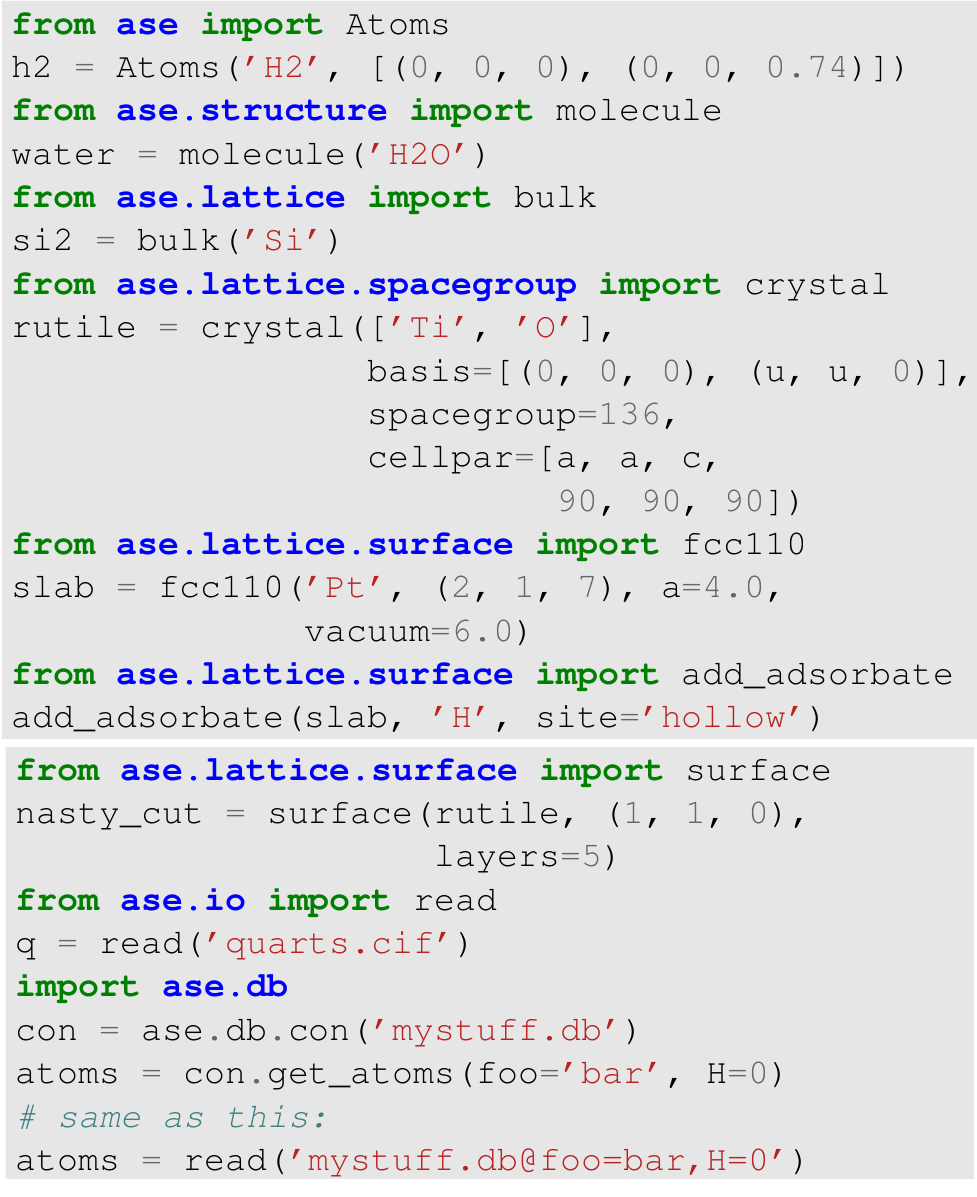
\includegraphics[height=2.9in,width=2.2in,viewport=0 0 970 1200,clip]{Figures/ASE_atoms_module-examples.png}
%\caption{\fontsize{7.2pt}{4.2pt}\selectfont{\textrm{The integrated calculator in ASE (Atomic Simulation Environment).}}}%
\label{Logo_atoms-module}
\end{figure} 
}

\frame
{
\frametitle{\textrm{ASE}特色:~软件接口丰富}
\textcolor{purple}{\textrm{ASE}}:~\textrm{Calculator}模块提供的可选的软件接口
\begin{figure}[h!]
\centering
\vspace*{-0.05in}
%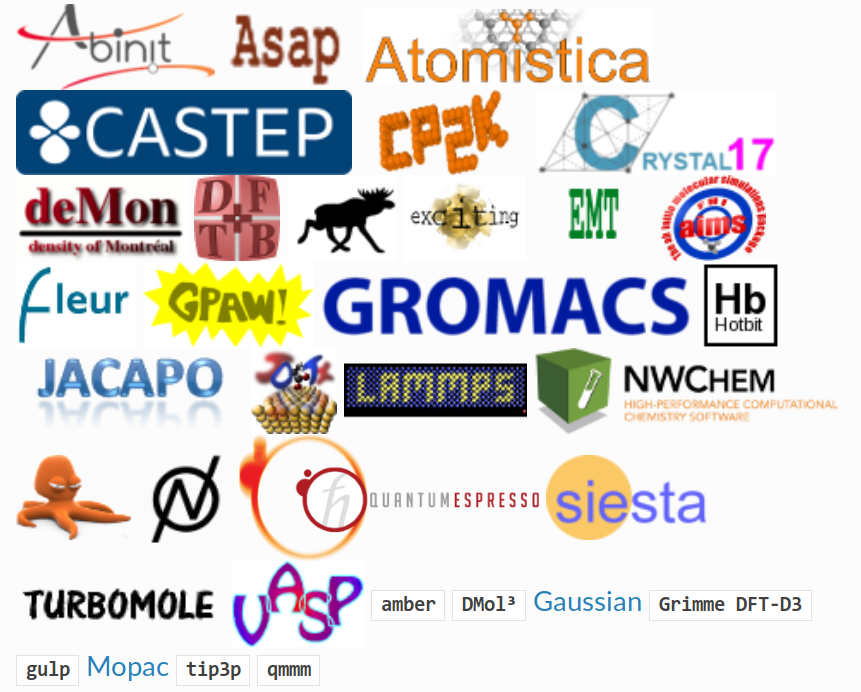
\includegraphics[height=1.0in,width=1.4in,viewport=0 0 638 530,clip]{Figures/ASE_calculator.png}
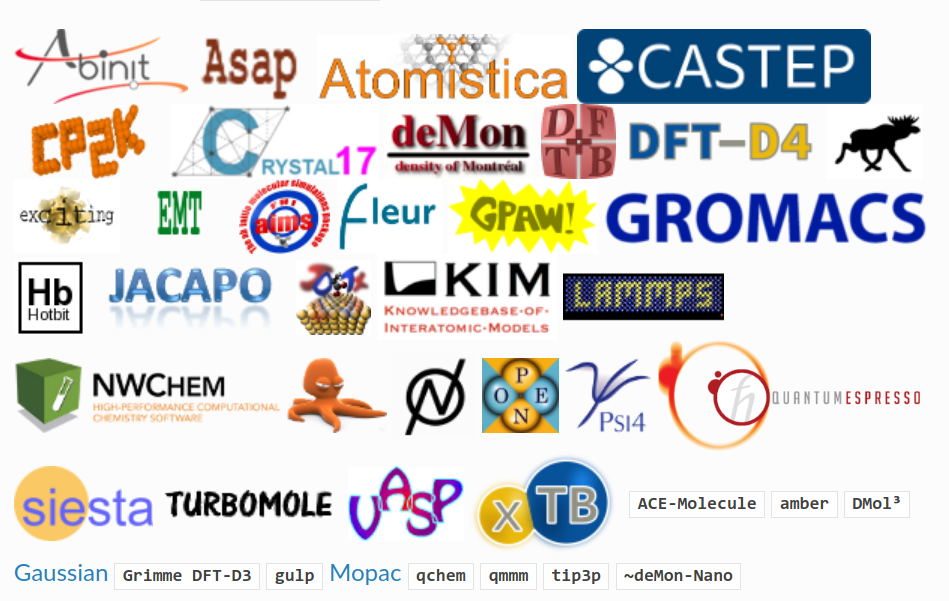
\includegraphics[height=2.0in,width=3.2in,viewport=0 0 940 600,clip]{Figures/ASE_calculator-new.png}
\caption{\fontsize{7.2pt}{4.2pt}\selectfont{\textrm{The integrated calculator in ASE.}}}%
\label{ASE_Calculator}
\end{figure} 
}

\frame
{
\frametitle{\textrm{ASE}特色:~提供多种优化算法模块和数据库}
\begin{figure}[h!]
\centering
\vspace*{-0.18in}
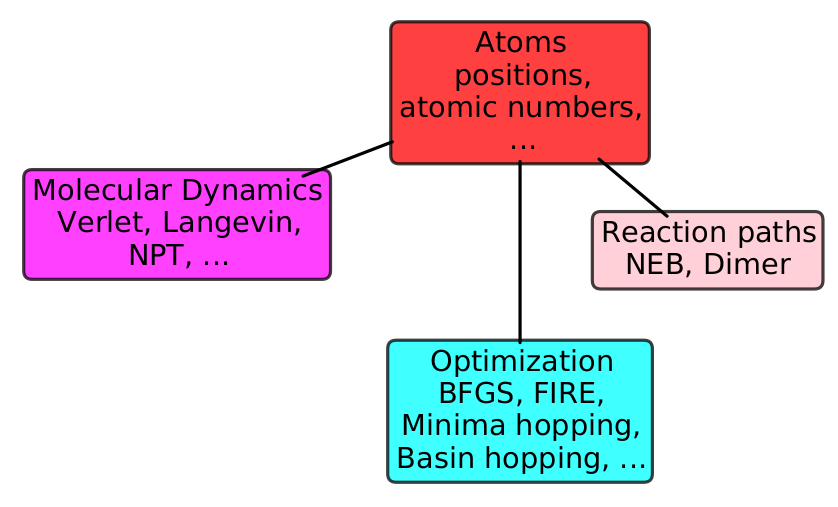
\includegraphics[height=1.3in,width=2.5in,viewport=0 0 838 500,clip]{Figures/ASE_opt_modules.png}
\vskip 1pt
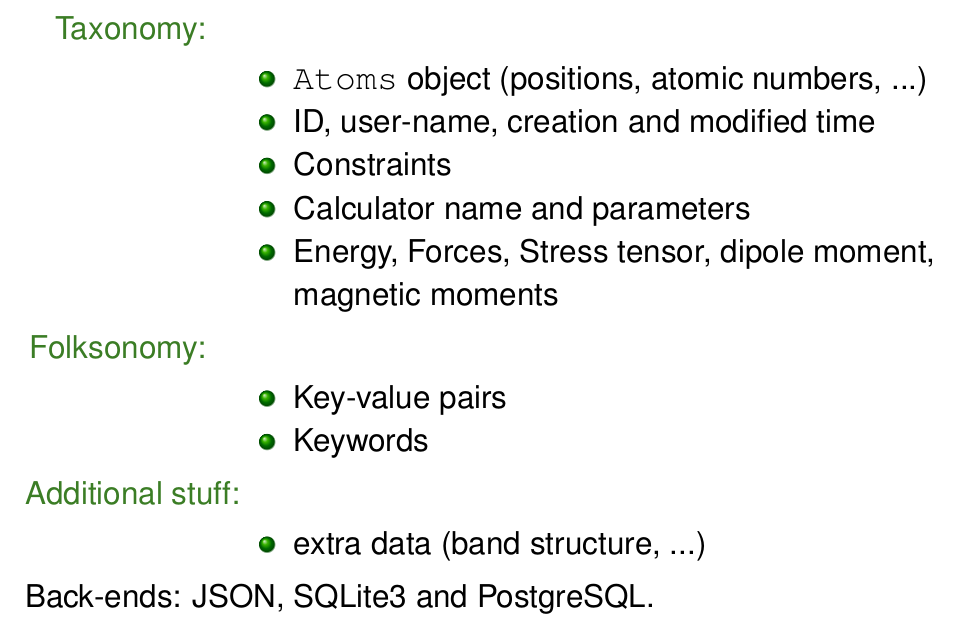
\includegraphics[height=1.7in,width=2.5in,viewport=0 0 938 630,clip]{Figures/ASE_database.png}
\label{ASE_opt-database}
\end{figure} 
}
%\frame
%{
%	\frametitle{\textrm{计算平台的作业自动提交:~基于\textrm{ASE}}}
%\begin{figure}[h!]
%\centering
%\vspace*{-0.2in}
%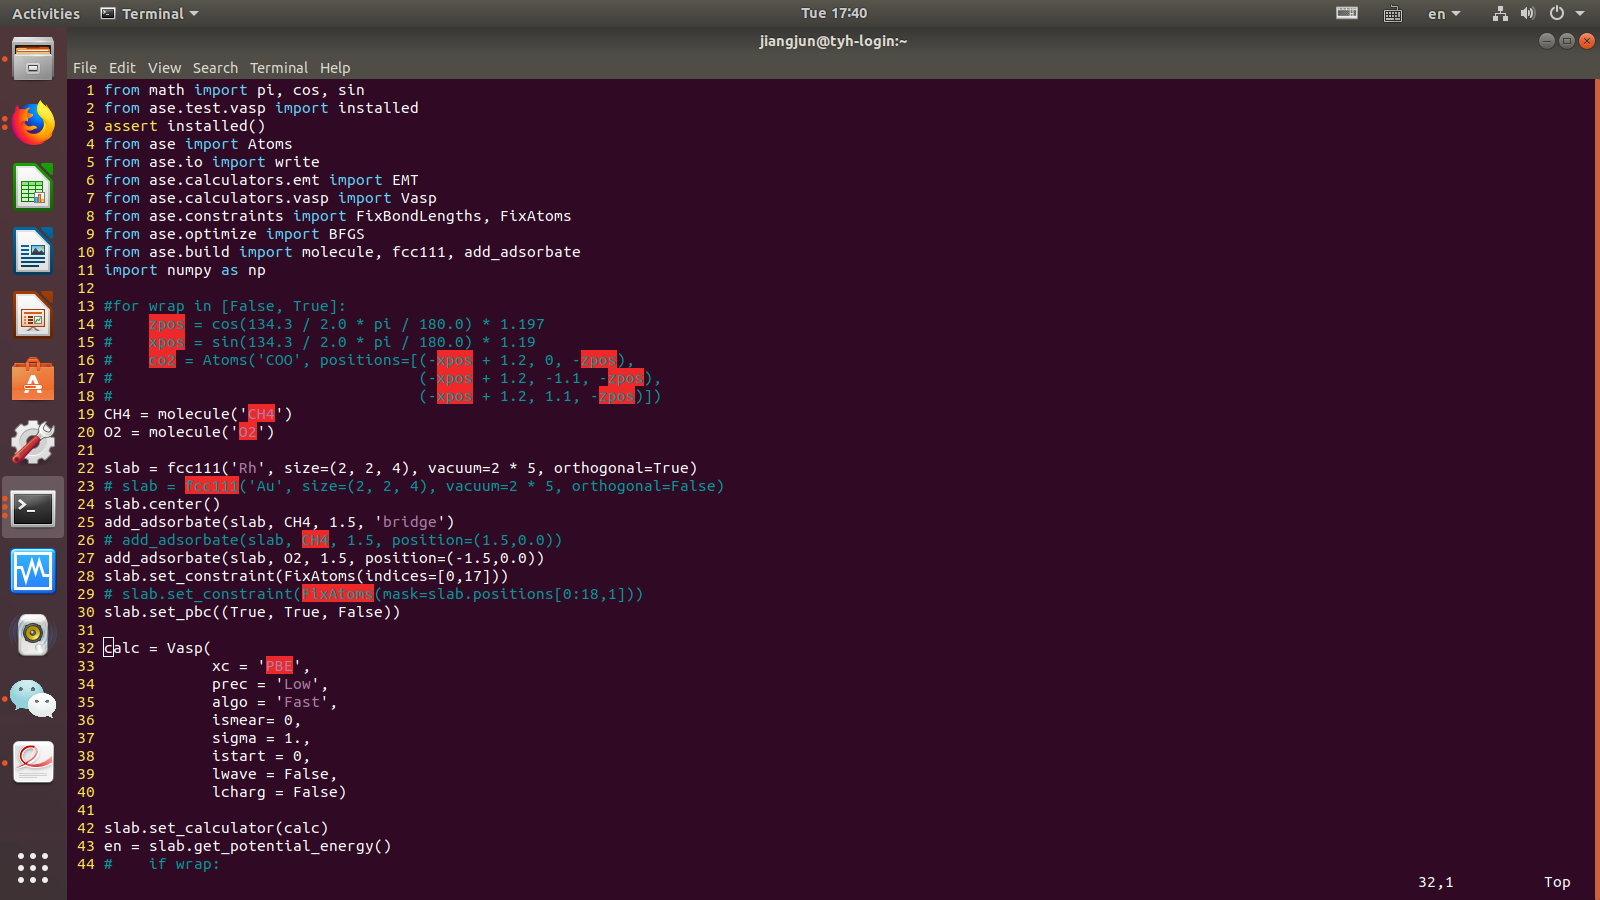
\includegraphics[height=3.1in,width=2.5in,viewport=75 0 725 820,clip]{Figures/ASE_app.png}
%%\caption{\fontsize{7.2pt}{4.2pt}\selectfont{\textrm{The integrated calculator in ASE (Atomic Simulation Environment).}}}%
%\label{ASE_app}
%\end{figure} 
%}

%\frame
%{
%	\frametitle{\textrm{计算平台的结果展示:~基于\textrm{MP}}}
%\begin{figure}[h!]
%\centering
%\vspace*{-0.2in}
%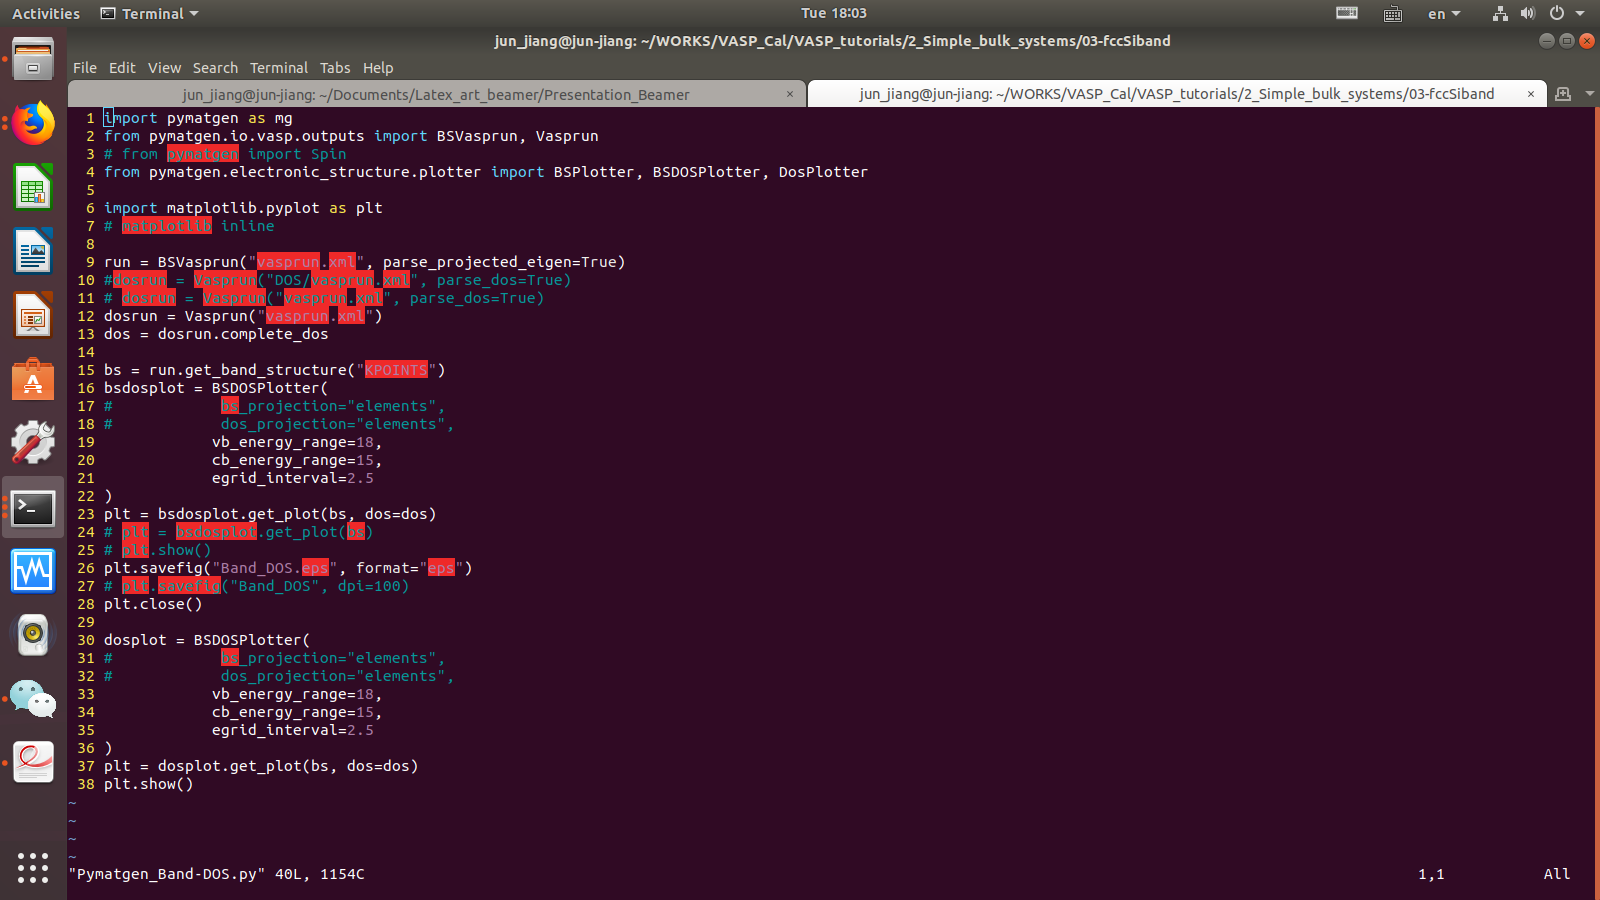
\includegraphics[height=3.1in,width=3.6in,viewport=73 80 880 790,clip]{Figures/Pymatgen_app.png}
%%\caption{\fontsize{7.2pt}{4.2pt}\selectfont{\textrm{The integrated calculator in ASE (Atomic Simulation Environment).}}}%
%\label{Pymatgen_app}
%\end{figure} 
%}
%

\frame
{
	\frametitle{计算平台的结果展示:~结合\textrm{MP}与\textrm{ASE}}
\begin{figure}[h!]
\centering
\vspace*{-0.2in}
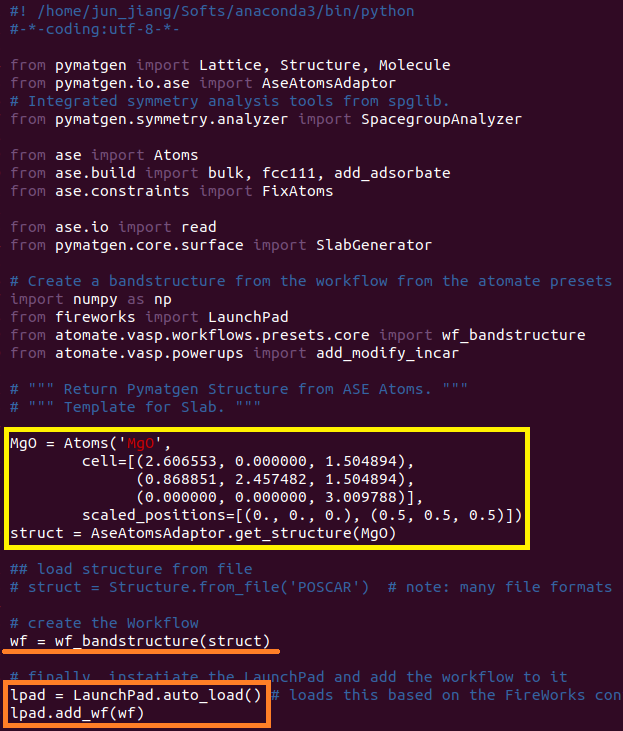
\includegraphics[height=3.0in,width=3.5in,viewport=0 0 600 550,clip]{Figures/Atomate-ASE_MgO.png}
%\caption{\fontsize{7.2pt}{4.2pt}\selectfont{\textrm{The integrated calculator in ASE (Atomic Simulation Environment).}}}%
\label{Atomate-ASE_app}
\end{figure} 
}

\frame
{
	\frametitle{应用示例:~\textrm{MgO:~DOS and Band}}
\begin{figure}[h!]
\centering
\vspace*{-0.16in}
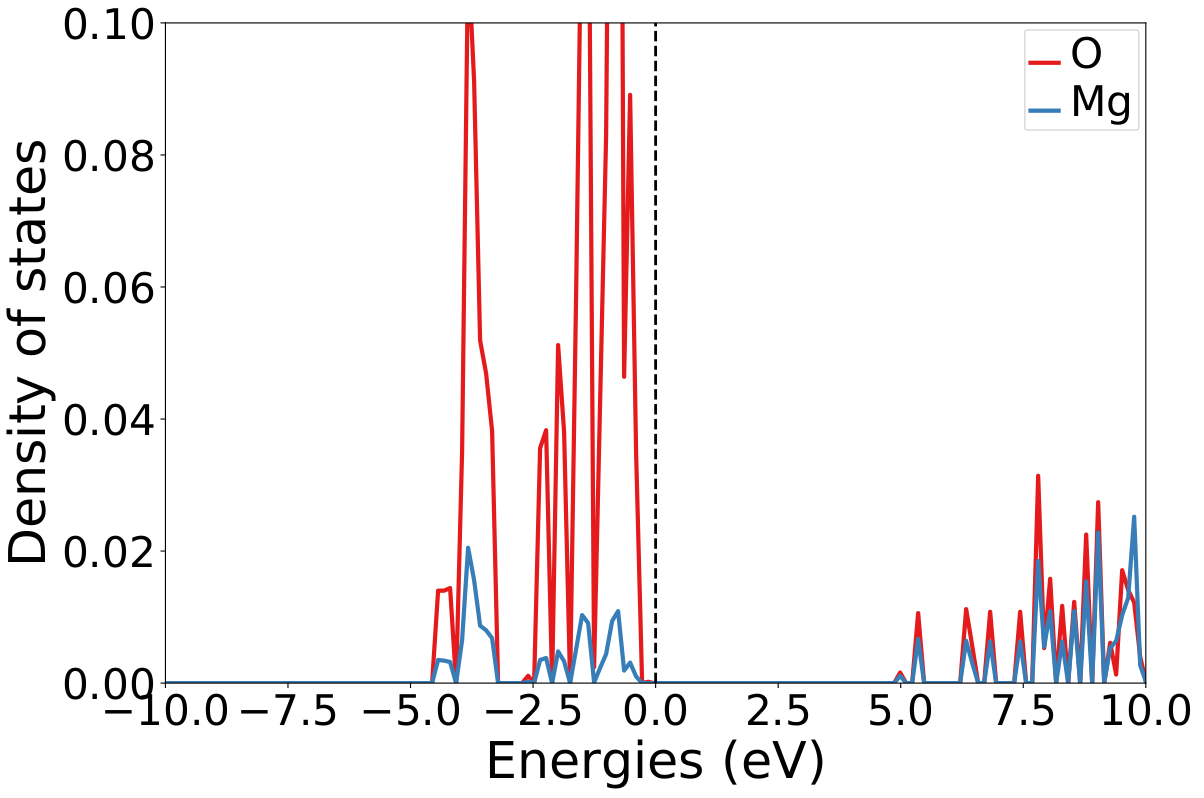
\includegraphics[height=1.5in,width=2.3in,viewport=0 0 900 600,clip]{Figures/Atomate_MgO-DOS.png}
\vskip 0.5pt
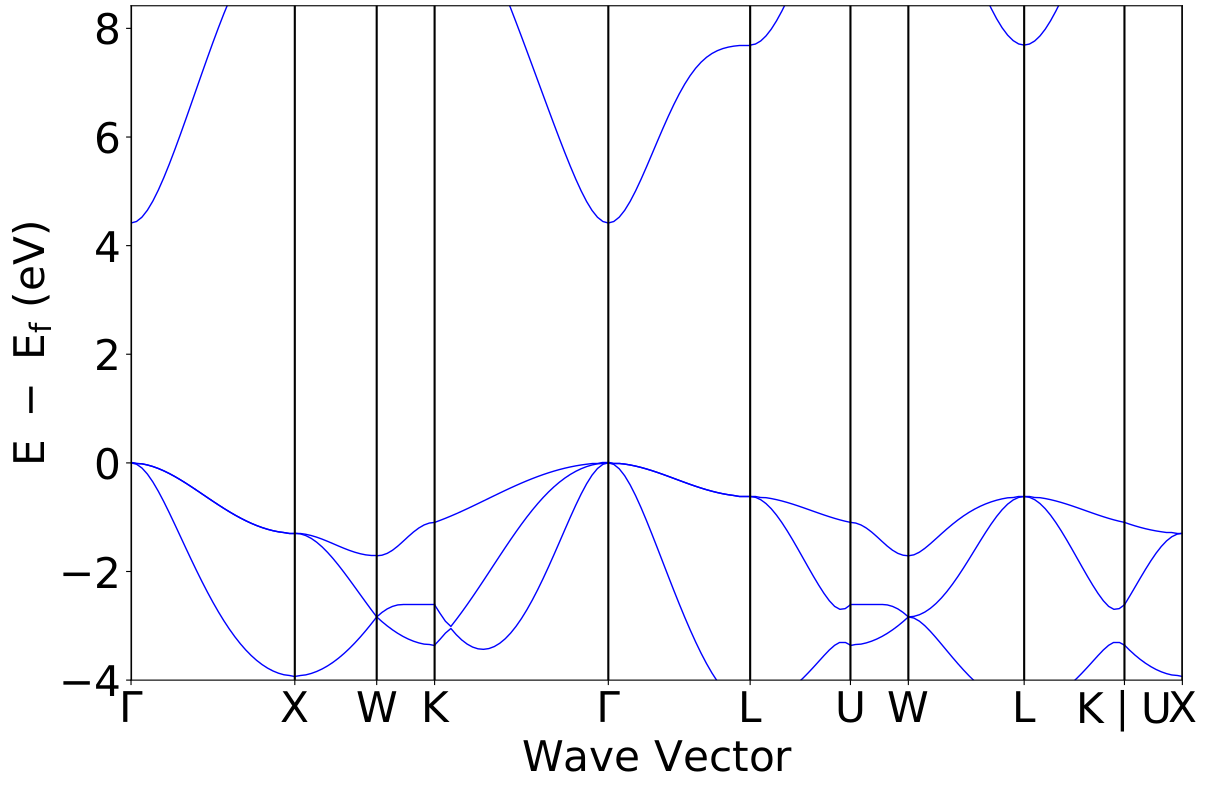
\includegraphics[height=1.5in,width=2.3in,viewport=0 0 900 600,clip]{Figures/Atomate_MgO-Band.png}
%\caption{\fontsize{7.2pt}{4.2pt}\selectfont{\textrm{The integrated calculator in Atomate-ASE.}}}%
\label{Atomate_MgO-DOS}
\end{figure} 
}

\frame
{
	\frametitle{材料数据库的功用:~发现新的材料}
\begin{figure}[h!]
\centering
\vspace*{-0.2in}
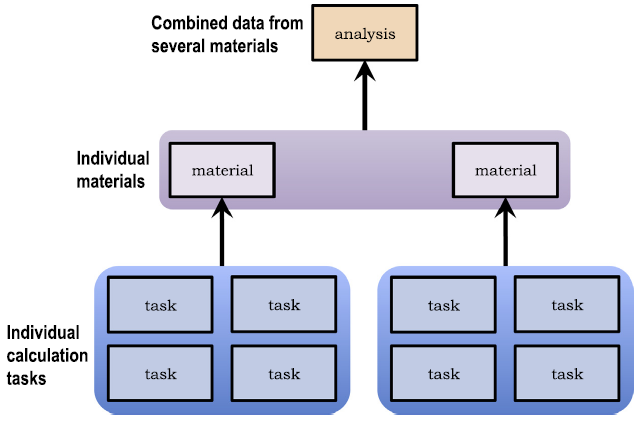
\includegraphics[height=2.6in,width=3.9in,viewport=0 0 640 440,clip]{Figures/MP_data.png}
%\caption{\fontsize{7.2pt}{4.2pt}\selectfont{\textrm{The integrated calculator in ASE (Atomic Simulation Environment).}}}%
\label{MP_data}
\end{figure} 
}

\begin{frame}
	\frametitle{适应异质界面催化模拟自动流程软件}
\begin{minipage}[c]{0.42\linewidth}
\begin{itemize}
\vspace*{-2.75in}
%	\item “标准化”对称性分析功能:~降低\textrm{DFT}的计算量
	\item \textcolor{blue}{前处理}:\\
		计算模型分析与预处理
%	\item \textcolor{magenta}{$\vec k\cdot\vec p$方法}:~提升电子计算的规模%,为\textrm{DFT-MD}计算提供基础
	\item \textcolor{blue}{计算流程设计与管理}:\\
		\begin{enumerate}
			\item 支持计算过程的模块化
			\item 支持高通量、跨尺度材料模拟
			\item 提供计算结果数据管理接口
		\end{enumerate}
	\item \textcolor{blue}{后处理}:\\
		结果数据的分析、挖掘与可视化展示
%	\item \textcolor{magenta}{机器学习}:~优化电子计算结果,获得\textrm{MD}尺度力场,\textrm{DFT-MD}耦合%,获得\textrm{MD}尺度下准确的多体相互作用的力场函数。
%	\item 设计合理完善的程序流程:~利用\textrm{MongoDB}支持的\textrm{FireWorks}计算流程管理%,由微观尺度\textrm{DFT}计算获得介观或宏观尺度的计算物性或者使不同尺度的计算结果更好地实现耦合自洽
\end{itemize}
\end{minipage}
\hskip 2pt
\begin{minipage}[b]{0.47\linewidth}
\begin{figure}[h!]
\centering
%\hskip -35pt
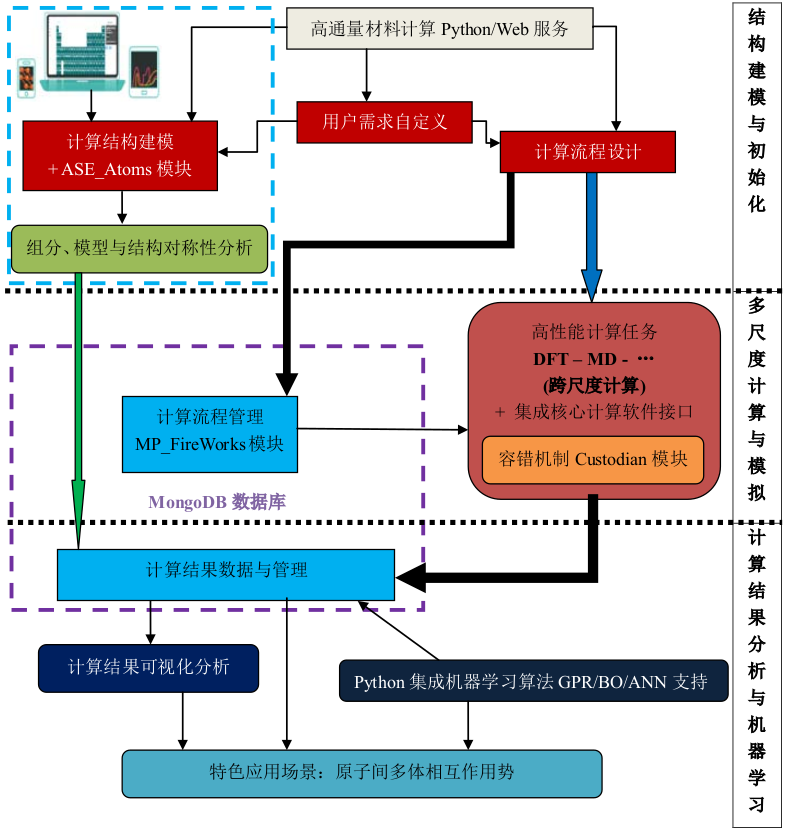
\includegraphics[height=2.18in]{Figures/MP_comp_BCC.png}
\caption{\fontsize{6.5pt}{4.5pt}\selectfont{适用于异质界面的高通量材料计算自动流程软件架构}}%
\label{MP_comp_BCC}
\end{figure}
\end{minipage}
\end{frame}

%------------------------------------------------------------------------Reference----------------------------------------------------------------------------------------------
%		\frame[allowframebreaks]
%{
%\frametitle{主要参考文献}
%\begin{thebibliography}{99}
%{\tiny
%	\bibitem{PR136-B864_1964}\textrm{P. Hohenberg and W. Kohn, \textit{Phys. Rev.} \textbf{136} (1964), B864}
%	\bibitem{PR140-A1133_1965}\textrm{W. Kohn and L.J. Sham, \textit{Phys. Rev.} \textbf{140} (1965), A1133}
%	\bibitem{PRB50-17953_1994}\textrm{P. E. Bl\"ochl. \textit{Phys. Rev.} B, \textbf{50} (1994), 17953}
%	\bibitem{PRB59-1758_1999}\textrm{G. Kresse and D. Joubert \textit{Phys. Rev.} B, \textbf{59} (1999), 1758}
%	\bibitem{Elect_Stru}\textrm{Richard. M. Martin. \textit{Electronic Structure: Basic Theory and Practical Methods} (Cambridge University Press, Cambridge, England, 2004)}
%        \bibitem{Singh}\textrm{D. J. Singh. \textit{Plane Wave, PseudoPotential and the LAPW method} (Kluwer Academic, Boston,USA, 1994)}					%
%}
%\end{thebibliography}
%%\nocite*{}
%}

\frame
{
\frametitle{主要参考文献}
\begin{thebibliography}{99}
\fontsize{6.5pt}{3.9pt}\selectfont{
	\bibitem{CMS58-227_2012}\textrm{S. Curtarolo, W. Setyawan, S. Wang, J. Xue, K. Yang, R. H. Taylor, L. J. Nelson, G. L. Hart, S. Sanvito, M. Buongiorno-Nardelli, N. Mingo and O. Levy \textit{Comp. Mater. Sci.}, \textbf{58} (2012), 227}
	\bibitem{CMS97-209_2015}\textrm{S. P. Ong, S. Cholia, A. Jain, M. Brafman, D. Gunter, G. Ceder and K. A. Persson. \textit{Comp. Mater. Sci.}, \textbf{97} (2015), 209}
	\bibitem{url_QMIP}\textrm{\url{http://www.qmip.org/qmip.org/Welcome.html}}
	\bibitem{JPCL2-2241_2011}\textrm{J. Hachmann, R. Olivares-Amaya, S. Atahan-Evrenk, C. Amador-Bedolla, R. S. S$\acute{a}$nchez-Carrera, A. Gold-Parker, L. Vogt, A. M. Brockway and A. Aspuru-Guzik \textit{J. Phys. Chem. Lett.}, \textbf{2} (2011), 2241}
%	\bibitem{url_Mater_Genome}\textrm{\url{https://www.whitehouse.gov/sites/default/files/microsites/ostp/materials_genome_initiative-final.pdf}}
	\bibitem{CMS146-319_2018}\textrm{X. Yang, Z. Wang, X. Zhao and H. Liu \textit{Comp. Mater. Sci.}, \textbf{146} (2018), 319}
	\bibitem{url_Matcloud}\textrm{\url{http://matcloud.cnic.cn}}
	\bibitem{CMS49-299_2010}\textrm{W. Setyawan and S. Curtarolo \textit{Comp. Mater. Sci.}, \textbf{49} (2010), 299}
	\bibitem{CMS50-2295_2011}\textrm{A. Jain, G. Hautier, C. J. Moore, S. P. Ong, C. C. Fischer, T. M. Kristin, K. A. Persson and G. Ceder \textit{Comp. Mater. Sci.}, \textbf{50} (2011), 2295}
%	\bibitem{unpublished}\textrm{D. Gunter, S. Cholia, A. Jain, M. Kocher, K. Persson, L. Ramakrishnan, S. P. Ong and G. Ceder. \textit{Community Accessible Datastore of High-Throughput Calculations: Experiences from the Materials Project} (unpublished)}
	\bibitem{MPC4-148_2015}\textrm{L. Lin \textit{Mater. Perform. Character.}, \textbf{4} (2015), 148}
}
\end{thebibliography}
\nocite*{}
}
%-----------------------------------------------------------------------------------------------------------------------------------------------------------------------%
